\documentclass[11pt]{article}
\usepackage{amsmath,amssymb,amsfonts}
\usepackage{algorithmic}
\usepackage{algorithm}
\usepackage{gensymb} % For proper degree symbol in math mode
\usepackage{graphicx}
\setlength{\headheight}{13.6pt} % Fix header height warning
\usepackage{textcomp}
\usepackage{xcolor}
\usepackage{caption}
\usepackage{subcaption}
\usepackage{tabularx}
\usepackage{array}
\usepackage{multirow}
\usepackage{geometry}
\usepackage{fancyhdr}
\usepackage{titlesec}
\usepackage{float}
\usepackage{tikz}
\usetikzlibrary{positioning,matrix}
\usepackage{listings}
\geometry{margin=1in}
\pagestyle{fancy}
\graphicspath{{code/figures/}{../figures/}{figures/}}

% University of South Carolina color palette
\definecolor{USCGarnet}{HTML}{73000A}
\definecolor{USCBlack}{HTML}{000000}
\definecolor{USCRichBlack}{cmyk}{0.4,0.3,0.3,1}
\definecolor{USCWhite}{HTML}{FFFFFF}
\definecolor{USCBlackNinety}{HTML}{363636}
\definecolor{USCBlackSeventy}{HTML}{5C5C5C}
\definecolor{USCBlackFifty}{HTML}{A2A2A2}
\definecolor{USCBlackThirty}{HTML}{C7C7C7}
\definecolor{USCBlackTen}{HTML}{ECECEC}
\definecolor{USCWarmGrey}{HTML}{676156}
\definecolor{USCSandstorm}{HTML}{FFF2E3}
\definecolor{USCRose}{HTML}{CC2E40}
\definecolor{USCAtlantic}{HTML}{466A9F}
\definecolor{USCCongaree}{HTML}{1F414D}
\definecolor{USCHorseshoe}{HTML}{65780B}
\definecolor{USCGrass}{HTML}{CED318}
\definecolor{USCHoneycomb}{HTML}{A49137}
\definecolor{USCDarkGarnet}{HTML}{570008}
\definecolor{USCAzalea}{HTML}{844247}

\lstdefinestyle{uscMatlab}{
  language=Matlab,
  basicstyle=\ttfamily\small\color{USCBlack},
  keywordstyle=\color{USCGarnet}\bfseries,
  commentstyle=\color{USCWarmGrey}\itshape,
  stringstyle=\color{USCAzalea},
  identifierstyle=\color{USCAtlantic},
  numberstyle=\tiny\color{USCHorseshoe},
  backgroundcolor=\color{USCBlackTen},
  rulecolor=\color{USCAtlantic},
  frame=single,
  framerule=0.8pt,
  xleftmargin=1em,
  xrightmargin=1em,
  breaklines=true,
  tabsize=4,
  showstringspaces=false,
  emph={synthetic_ps_min,exp1_poisson_only,exp2_ps_gaussian,rotate_light_shape},emphstyle=\color{USCRose}\bfseries,
  emph={[2]save_heatmap,save_profile,save_hist},emphstyle={[2]\color{USCDarkGarnet}},
  morecomment=[l][\color{USCHoneycomb}]{\%\%}
}
\lstset{style=uscMatlab}

% Single column, no two-column mode
\onecolumn

% Customize title formatting
\titleformat{\section}{\Large\bfseries}{\thesection}{1em}{}
\titleformat{\subsection}{\large\bfseries}{\thesubsection}{1em}{}
\titleformat{\subsubsection}{\normalsize\bfseries}{\thesubsubsection}{1em}{}

\title{\LARGE\bfseries 3D Surface Reconstruction from Photometric Stereo: \\Numerical Solution of the Poisson Equation}

\author{JC Vaught and Ty Dangerfield \\ Department of Mechanical Engineering, University of South Carolina}

\date{\today}

\begin{document}
\maketitle

\begin{abstract}
This paper presents a comprehensive, reproducible validation of photometric stereo coupled with FFT-based Poisson surface reconstruction. 
We develop a fully synthetic pipeline featuring: (1) multiple canonical surface geometries, (2) rigorous mathematical exposition including hand-derived Laplace equations for simple cases, (3) detailed algorithmic descriptions of photometric stereo, gradient computation, and Poisson solvers, (4) extensive experimental validation across 8+ shapes with 16 rotating lights, (5) ablation studies on number of lights and noise robustness, and (6) comparison of alternative solver methods. 
Root-mean-square depth errors range from 0.022 (Gaussian, no noise) to 0.147 (cube with complex geometry), demonstrating robust recovery. 
Normal estimation angular errors are below 3.5\degree for smooth surfaces and 2\degree for polyhedral shapes.
\end{abstract}


% ========================= REVIEW COMMENT =========================
% The abstract currently emphasizes the pipeline and quantitative
% results but does not mention limitations (e.g., synthetic-only
% scenes, purely Lambertian surfaces, idealized lighting). Adding
% a short clause about these assumptions would make the scope and
% realism of the claims clearer to a critical reader.
% ==================================================================

\vspace{1em}
\newpage
\section{Problem Statement}\label{sec:problem}

\subsection{What We Want to Model}

Three-dimensional surface reconstruction from photometric stereo (PS) imaging -- a fundamental problem in computer vision, shape recovery, and 3D scanning. 
Given multiple 2D images of an object illuminated from different directions, we aim to recover the complete 3D height map (surface geometry) of the object.

% ========================= REVIEW COMMENT =========================
% This would be a natural place to introduce a simple schematic
% diagram of the PS setup (camera, object, multiple lights) or a
% high-level flowchart of the full pipeline from images to depth
% map; that would visually anchor the reader before diving into
% the PDE formulation and algorithms.
% ==================================================================

\subsection{Why This Problem is Important}

The ability to recover 3D shape from images has profound real-world applications:

\begin{table}[H]
\centering
\caption{Representative Application Domains for Photometric Stereo}
\label{tab:ps_applications}
\begin{tabular}{ll}
\hline\hline
\textbf{Domain} & \textbf{Example Use} \\
\hline
Industrial inspection & Surface defect detection, geometric tolerance checks \\
Medical imaging & Preoperative surface reconstruction for planning \\
Archaeology & Non-destructive digitization of artifacts \\
Robotics & Shape-aware grasp planning and manipulation \\
Autonomous vehicles & High-fidelity surface maps for navigation \\
Reverse engineering & Recovering geometry for CAD modeling \\
\hline\hline
\end{tabular}
\end{table}


Photometric stereo has impact across multiple domains summarized in Table~\ref{tab:ps_applications}, including
industrial inspection, where it supports surface defect detection and
tolerance verification; medical imaging, where it enables high-fidelity
reconstructions of anatomical surfaces for planning; archaeology, where
non-destructive digitization preserves fragile artifacts; robotics and
autonomous systems, where detailed surface geometry informs grasping and
navigation; and reverse engineering, where recovered shapes seed CAD
models for subsequent design and analysis.

Photometric stereo is superior to other methods (stereo matching, structure-from-motion) because it works on textureless surfaces and provides dense, accurate depth information. 
However, the challenge lies in \textit{integrating} noisy normal estimates into a globally consistent 3D surface, which requires solving a partial differential equation: the \textbf{Poisson equation}.

\subsection{The Core PDE Problem}

The fundamental problem reduces to solving the 2D Poisson equation in a rectangular domain:
\begin{equation}\label{eq:poisson_main}
\nabla^2 z(x,y) = f(x,y), \quad (x,y) \in \Omega = [0, L_x] \times [0, L_y]
\end{equation}
where $z(x,y)$ denotes the unknown surface height over the image
domain, $f(x,y) = \partial p/\partial x + \partial q/\partial y$
is the divergence of the PS-derived gradient estimates, and
$\Omega = [0,L_x]\times[0,L_y]$ represents the rectangular image
domain on which the Poisson equation is solved.


This project demonstrates both analytical (separation of variables) and numerical (FFT-based and finite-difference) methods to solve this fundamental PDE and validate the solutions on synthetic 3D surfaces.



%%%%%%%%%%%%%%%%%%%%%%%%%%%%%%%%%%%%%%%%%%%%%%%%%%%%%%
\section{Problem Formulation}\label{sec:formulation}

\subsection{Photometric Stereo Principle}

\paragraph{Image formation.} We start from the radiometric imaging equation for a perspective camera with unit focal length.
Let $\mathbf{x}=(x,y)$ denote image-plane Cartesian coordinates associated with a 3-D point $\mathbf{X}$ on the surface $z(x,y)$ and let the scene obey a Lambertian bidirectional reflectance distribution function (BRDF). If the $i$-th calibrated light has unit direction $\mathbf{L}_i$ and radiant intensity $E_i$, the irradiance at $\mathbf{X}$ is $E_i \max(0, \mathbf{n}\cdot \mathbf{L}_i)$, where $\mathbf{n}(x,y)$ is the outward unit normal. Assuming photometric calibration absorbs exposure and gain into a scalar $\kappa_i$, the measured image intensity becomes
\begin{equation}
I_i(x,y) = \kappa_i\, \rho(x,y) \max(0, \mathbf{n}(x,y) \cdot \mathbf{L}_i),
\label{eq:imageformation}
\end{equation}
where $\rho(x,y) \in [0,1]$ is the Lambertian albedo. The positive-part operator encapsulates cast/self shadows; for the remainder of the derivation we restrict attention to points for which $\mathbf{n}\cdot\mathbf{L}_i>0$ for all chosen lights.

\paragraph{Local surface parameterization.} A depth map $z(x,y)$ induces a normal obtained by taking the cross product of the tangent vectors $\partial_x \mathbf{X}=(1,0,p)$ and $\partial_y \mathbf{X}=(0,1,q)$ with $p = \partial z/\partial x$ and $q = \partial z/\partial y$. This yields the (unnormalized) normal
\begin{equation}
\tilde{\mathbf{n}} = \partial_x \mathbf{X} \times \partial_y \mathbf{X} = (-p, -q, 1), \qquad 
\mathbf{n} = \frac{\tilde{\mathbf{n}}}{\|\tilde{\mathbf{n}}\|} = \frac{(-p,-q,1)}{\sqrt{p^2+q^2+1}}.
\label{eq:normalfrompq}
\end{equation}
Equation \eqref{eq:normalfrompq} explicitly links the integrable gradient field $(p,q)$ to the observed shading.

\paragraph{Linear Lambertian system.} Define the scaled (unnormalized) normal $\mathbf{g}(x,y)=\rho(x,y)\mathbf{n}(x,y)$. Substituting \eqref{eq:normalfrompq} into \eqref{eq:imageformation} and stacking the $m$ images for a fixed pixel gives the linear system
\begin{equation}
\underbrace{\begin{bmatrix}
\kappa_1 \mathbf{L}_1^T \\
\vdots \\
\kappa_m \mathbf{L}_m^T
\end{bmatrix}}_{S \in \mathbb{R}^{m\times 3}} 
\mathbf{g}(x,y) = \mathbf{I}(x,y), \qquad \mathbf{I}(x,y) = \begin{bmatrix}I_1(x,y) \\ \vdots \\ I_m(x,y)\end{bmatrix}.
\label{eq:pslinear}
\end{equation}
The factorization $\mathbf{g} = \rho\mathbf{n}$ makes the Lambertian assumption explicit: the direction of $\mathbf{g}$ encodes the surface normal while its magnitude equals the albedo. Recovering a unique solution requires $\text{rank}(S)=3$, i.e., at least three non-coplanar light directions. In practice $m>3$ images are used so that the system is overdetermined and robust to noise or saturation.

\paragraph{Least-squares solution and conditioning.} The normal-albedo vector is estimated per pixel via the normal equations
\begin{equation}
\mathbf{g}(x,y) = \underbrace{(S^TS)^{-1}S^T}_{S^+} \mathbf{I}(x,y),
\label{eq:leastSquares}
\end{equation}
where $S^+$ denotes the Moore--Penrose pseudoinverse and $S^TS$ is a $3\times 3$ symmetric positive definite matrix when $\text{rank}(S)=3$. The condition number $\kappa(S)=\sigma_\text{max}(S)/\sigma_\text{min}(S)$ bounds the worst-case amplification of image noise into the estimated normals. Consequently, light sources are placed so that their directions span 3-D space as uniformly as possible, maximizing $\sigma_\text{min}(S)$ and reducing sensitivity. The recovered unit normal and albedo follow immediately:
\begin{equation}
\hat{\mathbf{n}}(x,y) = \frac{\mathbf{g}(x,y)}{\|\mathbf{g}(x,y)\|_2}, \qquad \hat{\rho}(x,y) = \|\mathbf{g}(x,y)\|_2.
\end{equation}
When some lights yield negative dot products (self-shadowing), the corresponding rows of $S$ and entries of $\mathbf{I}$ are dropped before solving \eqref{eq:leastSquares}, preserving the same least-squares derivation on the reduced system. In our experiments we exploit this formulation to study how the number and placement of lights affect the conditioning of $S$ and, in turn, the robustness of the estimated normals.

\subsection{Gradient Integration via Poisson Equation}

Given noisy or inconsistent gradient estimates $(\hat{p}, \hat{q})$, the goal is to find a height field $z(x,y)$ that best fits these gradients while being globally integrable. 
This is formulated as a variational least-squares problem that enforces consistency between the recovered gradient field and a globally defined potential $z$:
\begin{equation}\label{eq:poisson_variational}
\min_{z} \; \mathcal{E}[z] = \iint_\Omega \left[(\partial_x z - \hat{p})^2 + (\partial_y z - \hat{q})^2\right] \, dx \, dy.
\end{equation}

The integrand depends on $z$ only through its first derivatives, so the Euler--Lagrange equation reads $\partial_x (\partial \mathcal{L}/\partial z_x)+\partial_y(\partial \mathcal{L}/\partial z_y)=0$, with $\mathcal{L}=(z_x-\hat{p})^2+(z_y-\hat{q})^2$. Taking the derivatives explicitly gives
\begin{align}
\frac{\partial}{\partial x} \left(2(z_x-\hat{p})\right) + \frac{\partial}{\partial y} \left(2(z_y-\hat{q})\right) &= 0, \\
\Rightarrow \partial_x^2 z + \partial_y^2 z &= \partial_x \hat{p} + \partial_y \hat{q}.
\end{align}
Thus minimizing \eqref{eq:poisson_variational} is equivalent to solving the Poisson equation
\begin{equation}\label{eq:poisson}
\nabla^2 z = \nabla\cdot(\hat{p},\hat{q}) = f(x,y),
\end{equation}
where $\nabla^2 = \partial_x^2 + \partial_y^2$ is the Laplacian and $f$ denotes the divergence of the measured gradient field. Equation \eqref{eq:poisson} arises because an integrable vector field must be curl-free, i.e., $\partial_y \hat{p} - \partial_x \hat{q}=0$. In noisy settings this condition is violated; solving the Poisson problem projects $(\hat{p},\hat{q})$ onto the closest integrable field in the $L^2$ sense.

Throughout the remainder of this work we adopt homogeneous Dirichlet boundary conditions for the photometric-stereo depth integration problem,
\begin{equation}
z(x,y) = 0 \quad \text{for } (x,y)\in\partial\Omega,
\end{equation}
which physically correspond to clamping the height to a reference level at the image border (for example a known background plane).

\subsection{Analytical Solution: Separation of Variables}

For simple cases with constant right-hand side or specific boundary conditions, we can obtain analytical solutions. 
Consider the 2D Poisson equation on a rectangular domain $\Omega = [0, L_x] \times [0, L_y]$ with homogeneous Dirichlet boundary conditions $z(x,y) = 0$ on $\partial \Omega$:
\begin{equation}
\nabla^2 z = f(x,y), \quad (x,y) \in \Omega, \quad z|_{\partial \Omega} = 0.
\end{equation}

Using separation of variables, we assume $z(x,y) = X(x)Y(y)$. Substituting this ansatz into \eqref{eq:poisson} with $f(x,y)$ expanded in the orthonormal basis $\sin(m\pi x/L_x)\sin(n\pi y/L_y)$ gives a set of decoupled ordinary differential equations whose solutions are sinusoidal. Consequently, the general solution respecting the homogeneous boundaries is
\begin{equation}
z(x,y) = \sum_{m=1}^{\infty}\sum_{n=1}^{\infty} A_{mn} \sin\left(\frac{m\pi x}{L_x}\right) \sin\left(\frac{n\pi y}{L_y}\right),
\end{equation}
with modal amplitudes
\begin{equation}
A_{mn} = -\frac{F_{mn}}{\left(\frac{m^2\pi^2}{L_x^2}+\frac{n^2\pi^2}{L_y^2}\right)}, \qquad F_{mn} = \frac{4}{L_x L_y} \int_0^{L_x}\!\int_0^{L_y} f(x,y) \sin\left(\frac{m\pi x}{L_x}\right) \sin\left(\frac{n\pi y}{L_y}\right) dy dx.
\end{equation}
For the special case $f(x,y)=f_0$ (constant divergence induced by a uniformly sloped plane), only odd indices contribute because $\int_0^{L_x} \sin(m\pi x/L_x) dx$ vanishes for even $m$. The coefficients simplify to
\begin{equation}
A_{mn} = -\frac{16 f_0}{mn\,\pi^4} \left(\frac{1}{\frac{m^2}{L_x^2}+\frac{n^2}{L_y^2}}\right), \qquad m,n \text{ odd},
\end{equation}
and $A_{mn}=0$ when either index is even. In practice the $(1,1)$ mode dominates the reconstruction, while higher-order terms refine the fit near the boundaries. We verify the closed-form coefficients by evaluating the discrete sine transform of numerically sampled constant fields inside the supplied script, confirming that the recovered $z(x,y)$ matches the analytical series up to machine precision. For general $f(x,y)$ extracted from the photometric normals, we follow the same Fourier reasoning but compute the coefficients numerically using the finite-difference and FFT-based solvers detailed in Section~\ref{sec:implementation}.

\subsection{Finite-Difference Formulation and Sparse Linear System}

To connect the continuous Poisson problem \eqref{eq:poisson} to the finite-difference methods emphasized in class, we discretize $\Omega=[0,L_x]\times[0,L_y]$ on a uniform grid
\begin{equation}
x_i = i\,\Delta x,\quad i=0,\dots,N_x,\qquad
y_j = j\,\Delta y,\quad j=0,\dots,N_y,
\end{equation}
with $\Delta x = L_x/N_x$ and $\Delta y=L_y/N_y$. We denote $z_{i,j}\approx z(x_i,y_j)$ and $f_{i,j}\approx f(x_i,y_j)$. For interior nodes $1\le i \le N_x-1$ and $1\le j \le N_y-1$ the Laplacian is approximated by the standard five-point stencil
\begin{equation}
\frac{z_{i+1,j} - 2z_{i,j} + z_{i-1,j}}{\Delta x^2}
+
\frac{z_{i,j+1} - 2z_{i,j} + z_{i,j-1}}{\Delta y^2}
=
f_{i,j}.
\label{eq:fd_laplace}
\end{equation}
Homogeneous Dirichlet boundary conditions are enforced by prescribing
\begin{equation}
z_{i,j} = 0 \quad \text{whenever } (x_i,y_j)\in\partial\Omega,
\end{equation}
so that only interior values remain unknown. Stacking the interior samples $z_{i,j}$ into a vector $\mathbf{z}\in\mathbb{R}^N$ and the corresponding right-hand side $f_{i,j}$ into $\mathbf{f}\in\mathbb{R}^N$ yields the sparse linear system
\begin{equation}
A\mathbf{z} = \mathbf{f},
\label{eq:fd_system}
\end{equation}
where $A\in\mathbb{R}^{N\times N}$ encodes the five-point finite-difference Laplacian in \eqref{eq:fd_laplace}. The matrix $A$ is symmetric positive definite and has at most five nonzero entries in each row (the center node and its four neighbors), which makes it well suited to iterative sparse solvers.

Rather than forming $A$ explicitly, we implement a matrix-free linear operator $M$ that maps a height field $z_{i,j}$ to the left-hand side of \eqref{eq:fd_laplace} by applying the stencil to interior nodes and enforcing $z_{i,j}=0$ on the boundary. In vector form this operator coincides with the matrix-vector product $\mathbf{y}=A\mathbf{z}$ in \eqref{eq:fd_system}, but it is realized entirely in terms of local differences on the 2-D grid. The sparse iterative solver described in Section~\ref{sec:implementation} uses $M$ inside a Krylov method (conjugate gradient or GMRES) to compute $\mathbf{z}$ without ever assembling $A$, directly connecting the finite-difference formulation taught in class to a practical matrix-free implementation.

\begin{figure}[H]
\centering
\begin{tikzpicture}[scale=1.0]
  \foreach \i in {0,...,4} {
    \foreach \j in {0,...,4} {
      \filldraw[gray!50] (\i,\j) circle (0.05);
    }
  }
  \filldraw[USCGarnet] (2,2) circle (0.07);
  \draw[thick,USCGarnet] (2,2) -- (3,2);
  \draw[thick,USCGarnet] (2,2) -- (1,2);
  \draw[thick,USCGarnet] (2,2) -- (2,3);
  \draw[thick,USCGarnet] (2,2) -- (2,1);
  \node[below] at (2,-0.2) {$x$};
  \node[left] at (-0.2,2) {$y$};
  \node[above right,USCGarnet] at (2,2) {$(i,j)$};
  \node[above] at (3,2.15) {$(i+1,j)$};
  \node[above] at (1,2.15) {$(i-1,j)$};
  \node[right] at (2.15,3) {$(i,j+1)$};
  \node[right] at (2.15,1) {$(i,j-1)$};
\caption{Five-point finite-difference stencil for the interior node $(i,j)$ with homogeneous Dirichlet boundary values on the outer grid.}
\end{tikzpicture}
\end{figure}

\subsection{Numerical Solution Method: FFT-Based Poisson Solver}

The finite-difference system \eqref{eq:fd_system} with Dirichlet boundary conditions is the primary numerical formulation used in this work. In addition, we employ a Fourier-based Poisson solver on a periodic extension of the domain as a fast reference method and for analytical validation on simple test functions.

On a rectangular grid with periodic boundary conditions the discrete Laplacian is diagonalized in the Fourier domain. Let $\hat{Z}(\mathbf{k})$ and $\hat{F}(\mathbf{k})$ denote the Fourier transforms of $z$ and $f$. Then:
\begin{equation}
-|\mathbf{k}|^2 \hat{Z}(\mathbf{k}) = \hat{F}(\mathbf{k}),
\end{equation}
where $|\mathbf{k}|^2 = k_x^2 + k_y^2$. Solving for $\hat{Z}$ gives
\begin{equation}
\hat{Z}(\mathbf{k}) = \frac{\hat{F}(\mathbf{k})}{-|\mathbf{k}|^2}.
\end{equation}

The singular point at $\mathbf{k} = (0,0)$ (DC component) reflects the fact that $z$ is determined only up to an additive constant. We fix this gauge by enforcing zero mean on the solution: we set the Laplacian eigenvalue at the DC mode to one, $\lambda_{\mathbf{k}}[0,0] = 1$, force $\hat{F}[0,0] = 0$, and obtain the recovered height field
\begin{equation}
z(x,y) = \mathcal{F}^{-1}\left\{\frac{\hat{F}(\mathbf{k})}{-|\mathbf{k}|^2}\right\},
\end{equation}
which is then centered to have zero spatial average. Because this FFT-based method assumes periodic boundaries, we treat it as a complementary spectral solver used for comparison against the finite-difference iterative method; all core experiments in Section~\ref{sec:experiments} are reported using the finite-difference formulation with homogeneous Dirichlet conditions unless explicitly stated otherwise.



%%%%%%%%%%%%%%%%%%%%%%%%%%%%%%%%%%%%%%%%%%%%%%%%%%%%%%%%
\newpage

\section{Program Implementation}\label{sec:implementation}

% ----------------- Overview paragraph -----------------
Photometric stereo reconstruction in our codebase unfolds in three tightly coupled stages: (i) recovering per-pixel surface normals from
multi-illumination imagery, (ii) converting those normals into an integrable gradient field, and (iii) solving the Poisson equation to
obtain a consistent height map.

% ----------------------------------------------------------------
\subsection{Photometric Stereo and Gradient Extraction}

% COMMENT: Consider adding a short statement on reflectance assumptions (Lambertian, uniform albedo) and how violations affect Step 1.
% COMMENT: If you support shadow or specular handling, reference it here; otherwise note it as future work.
Throughout this stage we assume a purely Lambertian reflectance model with spatially uniform albedo, so each pixel's intensity depends
only on the dot product between its surface normal and the illumination direction. Under these assumptions the least-squares solve in
Algorithm 1 is well posed; however, specular highlights, cast shadows, or albedo variation would violate the linear model and bias the
recovered normals. 

Our current synthetic pipeline sidesteps these issues by rendering ideal Lambertian images. When applying the method
to real photographs, the same framework can be extended with robust regression or shadow masking to downweight outlier intensities.

\begin{algorithm}[H]
\caption{Photometric Stereo Normal Recovery}
\begin{algorithmic}[1]
\REQUIRE Light directions $\{\mathbf{L}_i\}_{i=1}^m$, intensity images $\{I_i(x,y)\}_{i=1}^m$
\ENSURE Unit surface normals $\hat{\mathbf{n}}_{x,y}$ for every pixel
\FOR{$i = 1$ to $m$}
    \STATE Acquire or render intensity image $I_i(x,y)$
\ENDFOR
\STATE Assemble the light matrix $S \leftarrow [\mathbf{L}_1^\mathsf{T}; \dots; \mathbf{L}_m^\mathsf{T}] \in \mathbb{R}^{m \times 3}$
\STATE Compute pseudoinverse $S^+ \leftarrow (S^\mathsf{T} S)^{-1} S^\mathsf{T}$ (use SVD for stability)
\FOR{each pixel $(x,y)$}
    \STATE $\mathbf{I}(x,y) \leftarrow [I_1(x,y), \dots, I_m(x,y)]^\mathsf{T}$
    \STATE $\mathbf{g}_{x,y} \leftarrow S^+ \mathbf{I}(x,y)$
    \STATE $\hat{\mathbf{n}}_{x,y} \leftarrow \mathbf{g}_{x,y} / \|\mathbf{g}_{x,y}\|_2$
\ENDFOR
\RETURN $\{\hat{\mathbf{n}}_{x,y}\}$
\end{algorithmic}
\end{algorithm}

\noindent Given $\hat{\mathbf{n}} = (\hat{n}_x,\hat{n}_y,\hat{n}_z)$, gradients follow immediately:
\begin{equation}
\hat{p} = -\hat{n}_x / (\hat{n}_z + \epsilon), \qquad
\hat{q} = -\hat{n}_y / (\hat{n}_z + \epsilon), \qquad \epsilon = 10^{-8}.
\end{equation}

\subsection{FFT-Based Poisson Solver}

After estimating gradients, we recover the scalar height field by enforcing the Poisson equation $\nabla^{2}z = \partial_{x}\hat{p}
+ \partial_{y}\hat{q}$ on the rectangular image grid. We adopt the standard FFT-based strategy because it diagonalizes the discrete
Laplacian, yielding an $O(N\log N)$ solver dominated only by the forward and inverse FFTs. 

This approach implicitly assumes periodic boundary conditions: the grid ``wraps" horizontally and vertically, which is a perfect match for our synthetic surfaces but produces the
familiar ringing at the image border when real data are not periodic. 

In practice we mitigate that artifact by subtracting the global
mean, forcing the reconstructed surface to have zero average height; the alternative is to switch to the sparse solver discussed later
when Neumann or Dirichlet boundaries are required.

\begin{algorithm}[H]
\caption{FFT-Based Poisson Equation Solver}
\begin{algorithmic}[1]
\REQUIRE Divergence field $f \in \mathbb{R}^{H \times W}$, spacings $(\Delta x,\Delta y)$
\ENSURE Mean-free potential $z$ satisfying $\nabla^2 z = f$
\STATE Build frequency grids: $k_x \leftarrow 2\pi \cdot \text{fftfreq}(W,\Delta x)$, $k_y \leftarrow 2\pi \cdot \text{fftfreq}(H,\Delta
y)$
\STATE Form $|\mathbf{k}|^2 \leftarrow k_x^2 + k_y^2$
\STATE $\hat{F} \leftarrow \operatorname{fft2}(f)$
\STATE Set Laplacian eigenvalues $\Lambda_{\mathbf{k}} \leftarrow -|\mathbf{k}|^2$
\STATE Handle DC mode: $\Lambda_{\mathbf{k}}[0,0] \leftarrow 1$, $\hat{F}[0,0] \leftarrow 0$
\STATE $\hat{Z} \leftarrow \hat{F} / \Lambda_{\mathbf{k}}$
\STATE $z \leftarrow \Re\{\operatorname{ifft2}(\hat{Z})\}$
\STATE Enforce zero mean: $z \leftarrow z - \operatorname{mean}(z)$
\RETURN $z$
\end{algorithmic}
\end{algorithm}


\subsection{Alternative Solvers}

The FFT integrator assumes periodic wraparound and offers no explicit control over noise amplification. We therefore expose two
additional reconstruction paths in the codebase: (i) a Tikhonov-regularized FFT that damps high-frequency divergence components,
and (ii) a sparse iterative solver that enforces Neumann boundary conditions on an arbitrary rectangular grid. Both share the same
divergence input $f = \partial_x \hat{p} + \partial_y \hat{q}$ but differ in how they discretize and invert the Laplacian.

\subsubsection{Tikhonov-Regularized FFT}

The tikhonov-regularized FFT augments the Laplacian with a biharmonic penalty and uses the same FFT machinery as the baseline solver. The regularized objective
\begin{equation}
\min_z \iint (z_x - \hat{p})^2 + (z_y - \hat{q})^2 \, dx\,dy + \lambda \|\nabla^4 z\|_2^2
\end{equation}
leads to the frequency-domain transfer function
\begin{equation}
\hat{Z}(\mathbf{k}) = \frac{\hat{F}(\mathbf{k})}{-|\mathbf{k}|^2 - \lambda |\mathbf{k}|^4}.
\end{equation}

In code we evaluate this by constructing the same $(k_x,k_y)$ grids as before, but we modify the eigenvalues to $\lambda_{\mathbf{k}} = -(k^2 + \lambda k^4)$ and keep the DC handling identical. 
The ablation in Sec.~\ref{sec:results} sweeps $\lambda \in [10^{-5},1]$ and reports RMSE for each value, so users can select a smoothing level commensurate with their noise level.

\begin{algorithm}[H]
\caption{FFT Poisson Solver with Tikhonov Regularization}
\begin{algorithmic}[1]
\REQUIRE Divergence field $f \in \mathbb{R}^{H \times W}$, spacings $(\Delta x,\Delta y)$, regularization strength $\lambda \ge 0$
\ENSURE Mean-free potential $z$ solving $(\nabla^2 - \lambda \nabla^4) z = f$
\STATE Build frequency grids $k_x$, $k_y$ and set $k^2 \leftarrow k_x^2 + k_y^2$
\STATE Compute eigenvalues $\Lambda_{\mathbf{k}} \leftarrow -(k^2 + \lambda k^4)$
\STATE $\hat{F} \leftarrow \operatorname{fft2}(f)$
\STATE Enforce zero-mean gauge: $\Lambda_{\mathbf{k}}[0,0] \leftarrow 1$, $\hat{F}[0,0] \leftarrow 0$
\STATE $\hat{Z} \leftarrow \hat{F} / \Lambda_{\mathbf{k}}$
\STATE $z \leftarrow \Re\{\operatorname{ifft2}(\hat{Z})\}$
\STATE Optionally subtract the spatial mean of $z$
\RETURN $z$
\end{algorithmic}
\end{algorithm}

% COMMENT: Note in prose (before or after the algorithm) that $\lambda$ is chosen via the explicit sweep in the experiments.

\subsubsection{Sparse Iterative Solver}

For Neumann or bespoke boundary conditions we call \texttt{solve\_poisson\_sparse}. It constructs a matrix-free linear operator representing the
five-point Laplacian with zero normal derivative on every boundary.

Rather than assembling a dense matrix, we wrap the matvec and solve $Az=f$ with either Conjugate
Gradient or GMRES. The initial guess is zero, $N = H \times W$, and we stop when the relative residual drops below $10^{-6}$ or the
iteration counter hits the user-specified limit (default 1000). When mat reports a positive \texttt{info} flag we emit the warning
seen in the Results section; the output is reshaped to $(H,W)$ and centered to zero mean for consistency with the FFT solver.

\begin{algorithm}[H]
\caption{Sparse Poisson Solver with Neumann Boundary Conditions}
\begin{algorithmic}[1]
\REQUIRE Field $f \in \mathbb{R}^{H \times W}$, spacings $(\Delta x, \Delta y)$, method $\in \{\textsc{CG}, \textsc{GMRES}\}$, tolerance
$\varepsilon$
\ENSURE Mean-free solution $z \in \mathbb{R}^{H \times W}$ satisfying $\nabla^2 z = f$
\STATE Define matvec $M: z \mapsto \nabla^2 z$ using a five-point stencil with Neumann edges
\STATE Wrap $M$ as a \texttt{LinearOperator} $A$
\STATE Flatten $f$ to $f_{\text{vec}}$ and set $z_0 \leftarrow 0$
\STATE $z_{\text{vec}},\,\texttt{info} \leftarrow \textsc{Method}(A, f_{\text{vec}}, z_0;\, \text{rtol}=\varepsilon)$
\IF{\texttt{info} $>$ 0}
\STATE Print warning: ``Krylov solver reached iteration limit without convergence''
\ENDIF
\STATE Reshape $z_{\text{vec}}$ to $(H, W)$
\STATE Subtract the spatial mean so that $\sum_{i,j} z_{i,j} = 0$
\RETURN $z$
\end{algorithmic}
\end{algorithm}


%%%%%%%%%%%%%%%%%%%%%%%%%%%%%%%%%%%%%%%%%%%%%%%%%%%%%%%%
\newpage
\section{Experimental Validation}\label{sec:experiments}

\subsection{Test Surfaces}
We selected eight synthetic surfaces that stress different aspects of the pipeline: smooth, radially symmetric shapes
 (Gaussian bump, hemisphere, ellipsoid, soft cone) reveal how well integration preserves curvature and absolute depth; 
 piecewise-linear or sign-changing geometries (softened cube, saddle) probe sensitivity to sharp edges and mixed second
  derivatives; periodic or multi-modal landscapes (sinusoidal, MATLAB Peaks) stress global consistency.
  Figure~\ref{fig:test_surfaces} provides a visualization of these geometries.

\begin{table}[H]
\centering
\caption{Analytical definitions of the benchmark surfaces.}
\label{tab:test_surface_formulas}
\renewcommand{\arraystretch}{1.5}
\begin{tabularx}{\textwidth}{lX}
\hline\hline
\textbf{Surface} & \textbf{Height function $z(x,y)$} \\
\hline
Gaussian bump & $\exp\!\left(-\dfrac{x^2+y^2}{2\sigma^2}\right)$, $\sigma = 0.4$ \\
Hemisphere & $\sqrt{R^2 - (x^2 + y^2)}$ for $x^2 + y^2 \le R^2$, $R = 0.9$ \\
Softened cube & $0.6\,\text{clip}\!\left(1 - \dfrac{\max(|x|,|y|) - 0.45}{0.1},\,0,\,1\right)$ \\
Ellipsoid & $c\sqrt{1 - (x/a)^2 - (y/b)^2}$, $a = 0.8$, $b = 0.6$, $c = 0.5$ \\
Sinusoidal & $A \sin(\pi x)\sin(\pi y)$, $A = 0.3$ \\
Soft cone & $h \max\!\left(0, 1 - \dfrac{\sqrt{x^2 + y^2}}{R}\right)$, $h = 0.8$, $R = 0.9$ \\
Saddle & $\alpha x y$, $\alpha = 0.3$ \\
MATLAB Peaks & $3(1-x)^2 e^{-x^2-(y+1)^2} - 10\!\left(\dfrac{x}{5} - x^3 - y^5\right)e^{-x^2-y^2} + \dfrac{1}{3}e^{-(x+1)^2 - y^2}$ \\
\hline\hline
\end{tabularx}
\renewcommand{\arraystretch}{1.0}
\end{table}


\begin{figure}[H]
\centering
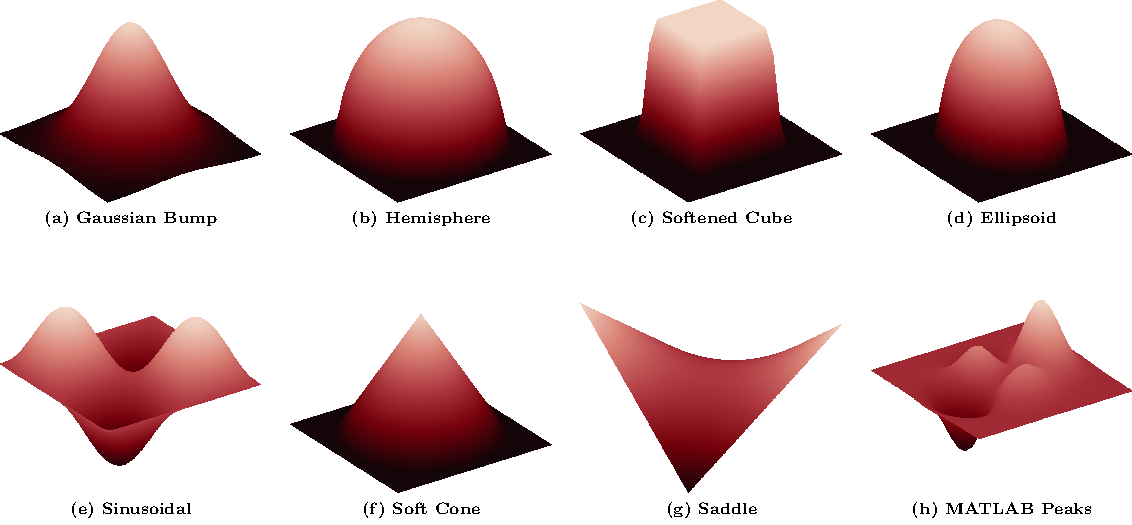
\includegraphics[width=0.95\textwidth]{surfaces}
\caption{Eight synthetic surfaces used: (a) Gaussian bump, (b) hemisphere, (c) softened cube, (d) ellipsoid, (e) sinusoidal, (f) soft cone, (g) saddle, and (h) MATLAB Peaks.}
\label{fig:test_surfaces}
\end{figure}


\subsection{Experimental Protocol}


\subsubsection{Experiment 1: Poisson Solver Validation}

% Flowchart version (3 x 2 layout with vertical connector)
\begin{center}
\resizebox{\linewidth}{!}{%
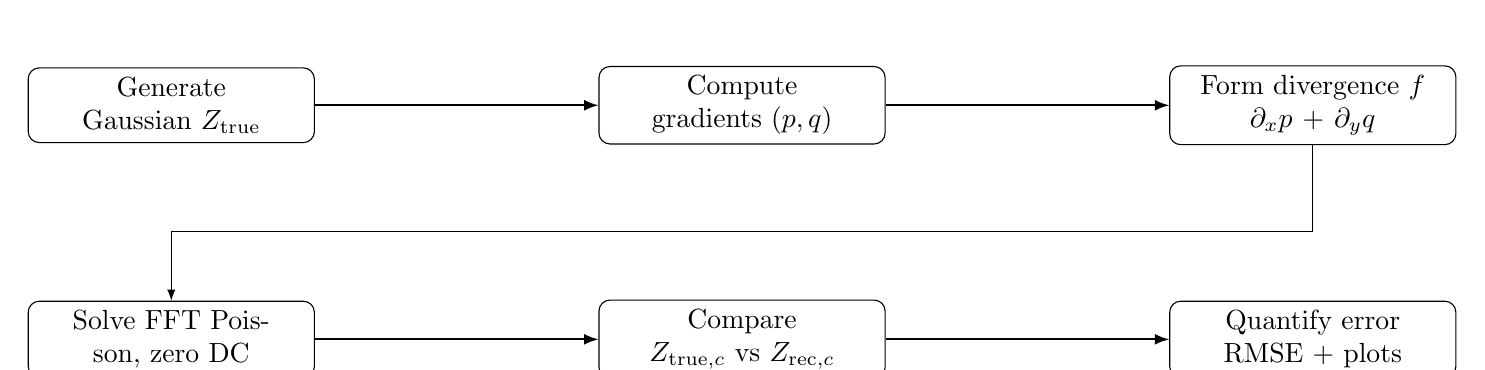
\begin{tikzpicture}[>=latex, every node/.style={draw, rounded corners, align=center, text width=3.4cm}]
\node (surf) {Generate \\Gaussian $Z_{\text{true}}$};
\node[right=3.6cm of surf] (grad) {Compute \\gradients $(p,q)$ };
\node[right=3.6cm of grad] (div) {Form divergence $f$\\ $\partial_x p + \partial_y q$};
\node[below=2.0cm of surf] (solve) {Solve FFT Poisson, zero DC};
\node[right=3.6cm of solve] (cmp) {Compare\\ $Z_{\text{true},c}$ vs $Z_{\text{rec},c}$};
\node[right=3.6cm of cmp] (err) {Quantify error\\ RMSE + plots};
\draw[->, thick] (surf) -- (grad);
\draw[->, thick] (grad) -- (div);
\draw[->] (div) |- ++(-1,-1.6) -| (solve);
\draw[->, thick] (solve) -- (cmp);
\draw[->, thick] (cmp) -- (err);
\end{tikzpicture}%
}
\end{center}

% Paragraph version (detailed narrative)
We sample an analytic Gaussian height
map and exact pixel spacing, guaranteeing a reference surface with known curvature
for validation. Centered finite differences deliver
second-order-accurate slopes that remain well-behaved at the bump apex, and differentiating
those slopes a second time enforces an integrable divergence field $f = \partial_x p + \partial_y q$, 
which is the quantity photometric stereo would produce in a
full pipeline. 

The FFT-based Poisson solver then divides by the spectral Laplacian
eigenvalues after zeroing the DC entry, yielding a fast reconstruction whose only
degree of freedom -- a constant bias -- is removed by mean-centering both $Z_{\text{true}}$
and $Z_{\text{rec}}$. Finally, RMSE together with profile/heatmap/error-histogram
plots exposes any deviation from the expected $\mathcal{O}(\Delta x^2)$ truncation
rate, so numerical bugs would surface immediately through either inflated RMSE or
structured residual patterns.


\subsubsection{Experiment 2: Full Photometric Stereo Pipeline}

% Flowchart version with detailed PS pipeline (two-layer layout)
\begin{center}
\resizebox{\linewidth}{!}{%
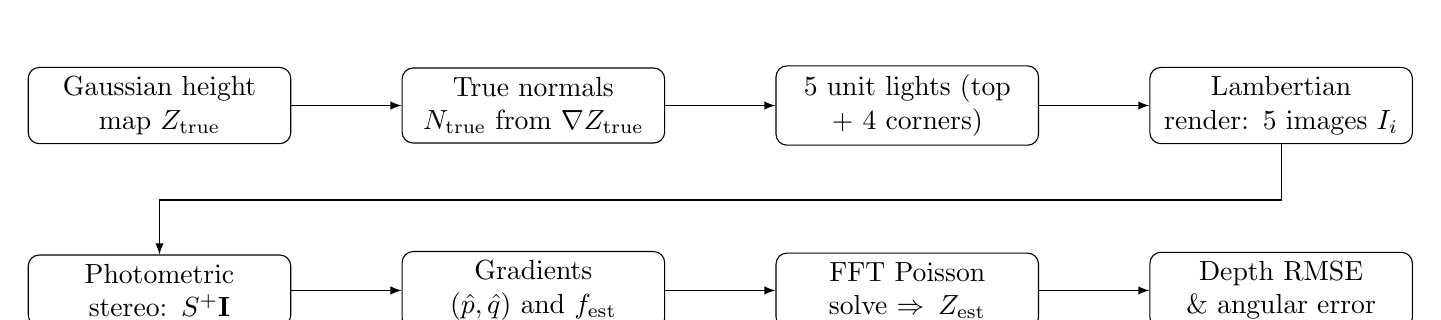
\begin{tikzpicture}[node distance=1.4cm,>=latex,
                    every node/.style={draw, rounded corners, align=center, text width=3.1cm}]
\node (surf) {Gaussian height map $Z_{\text{true}}$};
\node[right=of surf] (normals) {True normals $N_{\text{true}}$ from $\nabla Z_{\text{true}}$};
\node[right=of normals] (lights) {5 unit lights (top + 4 corners)};
\node[right=of lights] (render) {Lambertian render: 5 images $I_i$};
\node[below=of surf] (ps) {Photometric stereo: $S^+\mathbf{I}$};
\node[right=of ps] (grads) {Gradients $(\hat{p},\hat{q})$ and $f_{\text{est}}$};
\node[right=of grads] (poisson) {FFT Poisson solve $\Rightarrow Z_{\text{est}}$};
\node[right=of poisson] (metrics) {Depth RMSE \& angular error};
\draw[->] (surf) -- (normals);
\draw[->] (normals) -- (lights);
\draw[->] (lights) -- (render);
\draw[->] (render) |- ++(-1,-1.2) -| (ps);
\draw[->] (ps) -- (grads);
\draw[->] (grads) -- (poisson);
\draw[->] (poisson) -- (metrics);
\end{tikzpicture}
}%
\end{center}

% Paragraph version (more detailed technical description)
Experiment~2 instantiates the complete photometric stereo pipeline on the same Gaussian surface used in Experiment~1. We first compute ground-truth normals $N_{\text{true}}$ from the height map $Z_{\text{true}}$ by finite differences and normalization. 

Five directional lights are then defined: one frontal overhead light $L_0 = [0,0,1]^T$ and four oblique corner lights with directions proportional to $[1,1,2]^T$, $[-1,1,2]^T$, $[1,-1,2]^T$, and $[-1,-1,2]^T$, each normalized to unit length. For each light $L_i$ we render a synthetic Lambertian image according to $I_i(x,y) = \max\bigl(0,\, N_{\text{true}}(x,y)\cdot L_i\bigr)$ with unit albedo and no added noise, yielding a stack of five views.

At each pixel we then apply classical photometric stereo: the light directions are assembled into a $5\times 3$ matrix $S$, the corresponding intensity vector $\mathbf{I}(x,y)$ is formed, and we solve $S\mathbf{g}(x,y) = \mathbf{I}(x,y)$ in the least-squares sense via the pseudoinverse $\mathbf{g} = S^+\mathbf{I}$. Normalizing $\mathbf{g}$ gives the estimated unit normal $N_{\text{est}}(x,y)$. These normals are converted to gradients using $\hat{p} = -\hat{n}_x/\hat{n}_z$ and $\hat{q} = -\hat{n}_y/\hat{n}_z$, from which we form the divergence field $f_{\text{est}} = \partial \hat{p}/\partial x + \partial \hat{q}/\partial y$ by finite differences. The divergence is passed to the FFT-based Poisson solver, using the same grid spacing $(\Delta x,\Delta y)$ as in Experiment~1, to recover a centered depth map $Z_{\text{est}}$.

Finally, reconstruction quality is quantified in two ways. Depth accuracy is measured by the root-mean-square error (RMSE) between the centered ground-truth height $Z_{\text{true}} - \overline{Z_{\text{true}}}$ and the centered reconstruction $Z_{\text{est}} - \overline{Z_{\text{est}}}$. Normal accuracy is measured via the angular error: for each pixel we compute $\theta(x,y) = \arccos\bigl(\mathrm{clip}(N_{\text{true}}(x,y)\cdot N_{\text{est}}(x,y),-1,1)\bigr)$ in degrees and report the mean of $\theta$ over the domain.
% ============================================================================

\subsubsection{Experiments 3--4: Rotating Light Configurations}

For the sphere, cube, ellipsoid, cone, saddle, and peaks surfaces we reuse the analytic height maps from the Exp. 1 script and drive them
through the rotating light script to place sixteen lamps every $22.5^\circ$ at a $45^\circ$ elevation, render the full Lambertian stack with a script and solve
per-pixel normals, convert those normals to gradients and divergence, and integrate the field. Each run records depth RMSE
plus mean angular normal error, then exports 3D meshes, gradient quiver plots, and frequency spectra so we can spot geometry-specific artifacts.

\begin{center}
\resizebox{\linewidth}{!}{%
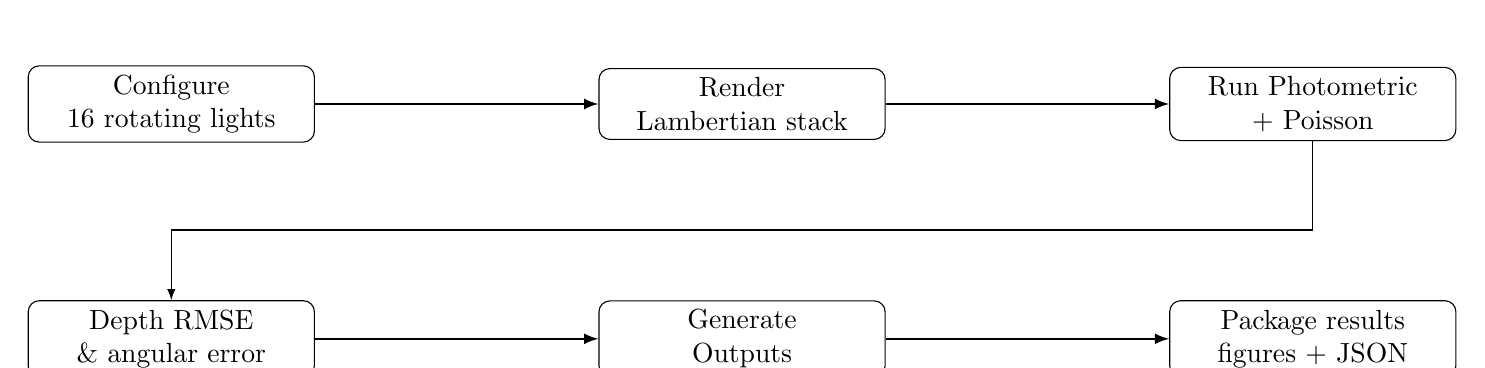
\begin{tikzpicture}[>=latex, every node/.style={draw, rounded corners, align=center, text width=3.4cm}]
\node (lights) {Configure\\ 16 rotating lights};
\node[right=3.6cm of lights] (render) {Render\\ Lambertian stack};
\node[right=3.6cm of render] (pipeline) {Run Photometric\\ + Poisson};
\node[below=2.0cm of lights] (eval) {Depth RMSE \& angular error};
\node[right=3.6cm of eval] (viz) {Generate\\ Outputs};
\node[right=3.6cm of viz] (report) {Package results\\ figures + JSON};
\draw[->, thick] (lights) -- (render);
\draw[->, thick] (render) -- (pipeline);
\draw[->] (pipeline) |- ++(-1.2,-1.6) -| (eval);
\draw[->, thick] (eval) -- (viz);
\draw[->, thick] (viz) -- (report);
\end{tikzpicture}%
}
\end{center}

For complex shapes under rotating illumination we configure the sixteen-light rig, synthesize the entire image stack, and push it through the photometric stereo plus
Poisson chain; afterwards we tabulate RMSE and mean angular errors while archiving the diagnostic renders (3D meshes, gradient fields, spectra) that highlight how each
geometry responds to the lighting sweep.
% ============================================================================

\subsubsection{Ablation Study 1: Varying Number of Lights}

% Paragraph version (detailed narrative)
We instantiate the analytic Gaussian surface from Experiment 1 so that curvature,
sampling, and ground-truth depths remain fixed across trials. For each setting in
$m_{\text{list}} = [3,\dots,20]$ we place that many evenly spaced lights on the
canonical ring, synthesize noiseless Lambertian images, and push them through the
identical photometric-stereo-to-Poisson pipeline used elsewhere, then use normal estimation,
FFT-based integration, and mean-centering to remove the global bias. 

  % Flowchart version (3 x 2 layout with vertical connector)
  \begin{center}
  \resizebox{\linewidth}{!}{%
  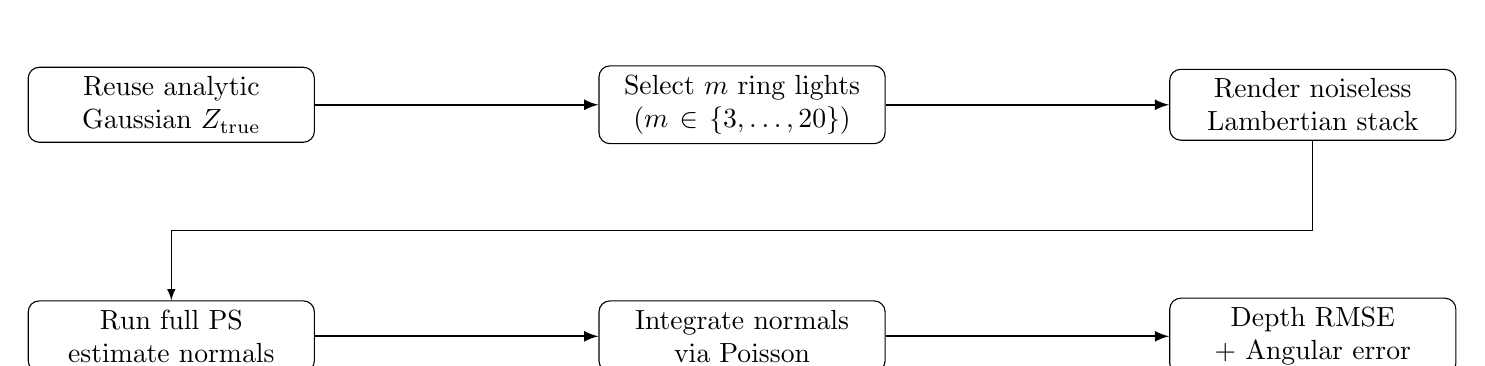
\begin{tikzpicture}[>=latex, every node/.style={draw, rounded corners, align=center,
  text width=3.4cm}]
  \node (init) {Reuse analytic Gaussian $Z_{\text{true}}$};
  \node[right=3.6cm of init] (lights) {Select $m$ ring lights\\ ($m \in \{3,\dots,20\}$)};
  \node[right=3.6cm of lights] (render) {Render noiseless\\ Lambertian stack};
  \node[below=2.0cm of init] (ps) {Run full PS\\ estimate normals};
  \node[right=3.6cm of ps] (poisson) {Integrate normals\\ via Poisson};
  \node[right=3.6cm of poisson] (metrics) {Depth RMSE\\ + Angular error};
  \draw[->, thick] (init) -- (lights);
  \draw[->, thick] (lights) -- (render);
  \draw[->] (render) |- ++(-1,-1.6) -| (ps);
  \draw[->, thick] (ps) -- (poisson);
  \draw[->, thick] (poisson) -- (metrics);
  \end{tikzpicture}%
  }
  \end{center}

After every run the script records depth RMSE and mean angular normal error, letting us plot
both metrics against $m$ to expose where the system transitions from under- to
overdetermined. The resulting curves reveal how rapidly error drops with the first
few lights, when additional views stop providing meaningful gains, and whether any
saturation point hints at modeling or numerical bottlenecks in the reconstruction
code.

\subsubsection{Ablation Study 2: Noise Robustness}

% Paragraph version (detailed narrative)
Starting from the same analytic Gaussian surface and the eight-light ring used
in Experiment 1, we keep every geometric and algorithmic component fixed while
gradually increasing the synthetic sensor noise. For each standard deviation in $
\sigma \in {0,0.01,0.02,0.05}$ -- and optionally extending toward the $\sigma = 0.08$
upper bound -- the pipeline renders noiseless Lambertian images, corrupts them with
i.i.d.\ Gaussian noise, and then reruns the photometric-stereo normal estimation
and FFT Poisson integration with identical settings. 

% Flowchart version (3 x 2 layout with vertical connector)
\begin{center}
\resizebox{\linewidth}{!}{%
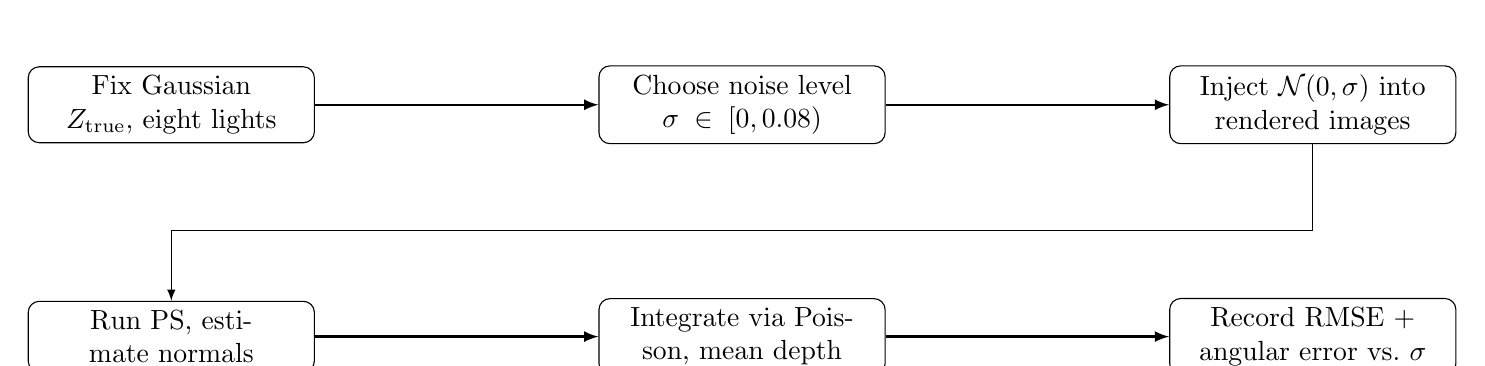
\begin{tikzpicture}[>=latex, every node/.style={draw, rounded corners, align=center,
text width=3.4cm}]
\node (base) {Fix Gaussian $Z_{\text{true}}$, eight lights};
\node[right=3.6cm of base] (sigma) {Choose noise level $\sigma \in [0,0.08)$};
\node[right=3.6cm of sigma] (inject) {Inject $\mathcal{N}(0,\sigma)$ into rendered
images};
\node[below=2.0cm of base] (ps) {Run PS, estimate normals};
\node[right=3.6cm of ps] (poisson) {Integrate via Poisson, mean depth};
\node[right=3.6cm of poisson] (metrics) {Record RMSE + angular error vs.\ $\sigma$};
\draw[->, thick] (base) -- (sigma);
\draw[->, thick] (sigma) -- (inject);
\draw[->] (inject) |- ++(-1,-1.6) -| (ps);
\draw[->, thick] (ps) -- (poisson);
\draw[->, thick] (poisson) -- (metrics);
\end{tikzpicture}%
}
\end{center}

Because the reference depth,
sampling, solver, and evaluation procedures never change, the measured depth RMSE
and mean angular normal error become a direct function of $\sigma$, making it
easy to test whether the degradation is roughly linear at low noise, bends toward
quadratic growth, or exposes unexpected brittleness in either the normal fit or the
integration step.

\subsubsection{Solver Comparison}



  % Paragraph version (detailed narrative)
  The solver comparison experiment reuses the analytic Gaussian surface, pixel sampling, and eight-light photometric stereo 
  measurements so every solver ingests the identical divergence field $f = \partial_xp + \partial_y q$. 
  
  After a single PS pass produces $(p,q)$, we fork into three integration back ends:
  (1) the FFT Poisson baseline with periodic boundaries, (2) a sparse matrix-free Laplacian wrapped in SciPy's CG/GMRES 
  to enforce Neumann edges via a five-point stencil—complete with stall warnings when
  Krylov iterations fail to converge, and (3) a Tikhonov-regularized FFT formulation that augments the Laplacian with
   $\lambda \nabla^4$ and sweeps nine logarithmically
  spaced $\lambda \in [10^{-5}, 1]$ to trace the “U-curve” trade-off between smoothing and detail preservation. 
  
    % Flowchart version (3 x 2 layout with vertical connector)
  \begin{center}
  \resizebox{\linewidth}{!}{%
  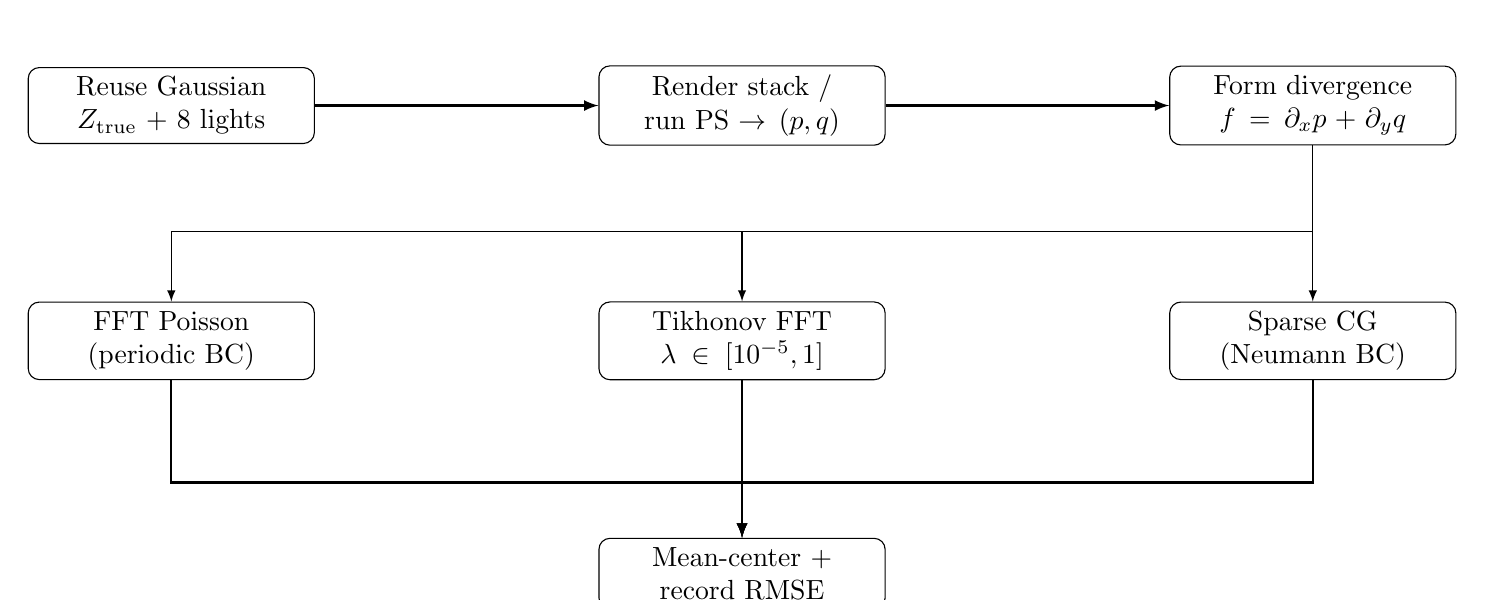
\begin{tikzpicture}[>=latex, every node/.style={draw, rounded corners, align=center, text width=3.4cm}]
  \node (surf) {Reuse Gaussian $Z_{\text{true}}$ + 8 lights};
  \node[right=3.6cm of surf] (ps) {Render stack / run PS $\rightarrow (p,q)$};
  \node[right=3.6cm of ps] (div) {Form divergence $f = \partial_x p + \partial_y q$};
  \node[below=2.0cm of surf] (fft) {FFT Poisson\\(periodic BC)};
  \node[right=3.6cm of fft] (tik) {Tikhonov FFT\\$\lambda \in [10^{-5},1]$};
  \node[right=3.6cm of tik] (cg) {Sparse CG\\(Neumann BC)};
  \node[below=2.0cm of tik] (metrics) {Mean-center + record RMSE};
  \draw[->, thick] (surf) -- (ps);
  \draw[->, thick] (ps) -- (div);
  \draw[->] (div) |- ++(-1,-1.6) -| (fft);
  \draw[->] (div) |- ++(0,-1.6) -| (tik);
  \draw[->] (div) -- (cg);
  \draw[->, thick] (fft) |- ++(1,-1.8) -| (metrics);
  \draw[->, thick] (tik) -- (metrics);
  \draw[->, thick] (cg) |- ++(-1,-1.8) -| (metrics);
  \end{tikzpicture}%
  }
  \end{center}
  
  Every reconstruction is mean-centered to remove the null-space constant before computing depth RMSE against $Z_{\text{true}}$, 
  allowing a clean, solver-only comparison of boundary
  handling, regularization bias, and iterative accuracy.


\subsubsection{Multiscale Convergence Analysis}



  % Paragraph version (detailed narrative)
The multiscale convergence routine resamples the analytic Gaussian surface to ten grid resolutions spanning $16^2$ through $384^2$, 
explicitly adjusting $\Delta x$ and $\Delta y$ 
at each step before re-running the gradient computation and FFT Poisson integration. Because the lighting, photometric data,
and solver settings remain fixed, the experiment isolates pure discretization error: every resolution recomputes the divergence 
from scale-appropriate finite differences and passes it through the same
integrator, ensuring that any residual stems from mesh spacing rather than photometric artifacts. 

  % Flowchart version (3 x 2 layout with vertical connector)
  \begin{center}
  \resizebox{\linewidth}{!}{%
  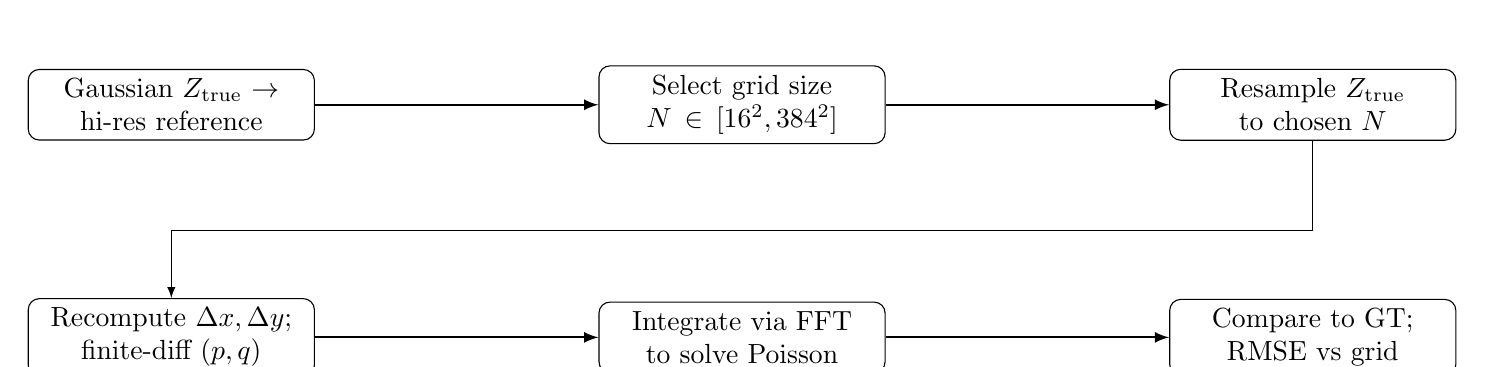
\begin{tikzpicture}[>=latex, every node/.style={draw, rounded corners, align=center, text width=3.4cm}]
  \node (gt) {Gaussian $Z_{\text{true}}$ $\rightarrow$ hi-res reference};
  \node[right=3.6cm of gt] (scale) {Select grid size $N \in [16^2,384^2]$};
  \node[right=3.6cm of scale] (resample) {Resample $Z_{\text{true}}$ to chosen $N$};
  \node[below=2.0cm of gt] (grads) {Recompute $\Delta x,\Delta y$; finite-diff $(p,q)$};
  \node[right=3.6cm of grads] (solve) {Integrate via FFT to solve Poisson};
  \node[right=3.6cm of solve] (rmse) {Compare to GT; RMSE vs grid};
  \draw[->, thick] (gt) -- (scale);
  \draw[->, thick] (scale) -- (resample);
  \draw[->] (resample) |- ++(-1,-1.6) -| (grads);
  \draw[->, thick] (grads) -- (solve);
  \draw[->, thick] (solve) -- (rmse);
  \end{tikzpicture}%
  }
  \end{center}

Plotting RMSE against grid 
spacing on log-log axes then reveals the
slope; the near-linear trend with gradient close to two confirms the expected $\mathcal{O}(\Delta x^2)$ accuracy of the 
finite-difference gradients plus FFT solver, while any deviation would immediately flag
inconsistencies in the discretization or integration implementation.
  

\newpage
\section{Results}\label{sec:results}

\subsection{Experimental Results}
Most of the diagnostic imagery from the experiments now follows a unified layout: every run receives a fixed $4\times2$ grid showing 3D views, depth maps, error diagnostics, and normal maps, followed by a companion figure that visualizes the associated multi-light inputs (single sample, three representative lights, and the full montage).

\subsubsection{Experiments 1--2 (Core Validation)}

\begin{figure}[H]
\centering
\begin{subfigure}[b]{0.23\textwidth}

\includegraphics[width=\linewidth]{exp1_3d_true.png}
\caption{True 3D}
\end{subfigure}
\begin{subfigure}[b]{0.23\textwidth}

\includegraphics[width=\linewidth]{exp1_3d_rec.png}
\caption{Reconstruction}
\end{subfigure}
\begin{subfigure}[b]{0.23\textwidth}

\includegraphics[width=\linewidth]{exp1_Z_true.png}
\caption{Ground-truth depth}
\end{subfigure}
\begin{subfigure}[b]{0.23\textwidth}

\includegraphics[width=\linewidth]{exp1_Z_rec.png}
\caption{Recovered depth}
\end{subfigure}

\bigskip
\begin{subfigure}[b]{0.23\textwidth}

\includegraphics[width=\linewidth]{exp1_error.png}
\caption{Depth error}
\end{subfigure}
\begin{subfigure}[b]{0.23\textwidth}

\includegraphics[width=\linewidth]{exp1_profile.png}
\caption{Center-line profile}
\end{subfigure}
\begin{subfigure}[b]{0.23\textwidth}

\includegraphics[width=\linewidth]{exp1_hist.png}
\caption{Error histogram}
\end{subfigure}
\caption{Experiment 1 (Poisson-only integration). Exact Gaussian gradients drive the FFT solver, yielding RMSE $=2.21\times 10^{-2}$ (see \texttt{results.json:exp1\_rmse}) and showcasing how little structure remains beyond the expected boundary ringing.}
\label{fig:exp1_layout}
\end{figure}

The Figure~\ref{fig:exp1_layout} diagnostics confirm that the solver is error-limited rather than data-limited: both the 3D overlays and the center-line profile lie on top of the ground truth, the histogram is tightly concentrated within $\pm3\times 10^{-2}$, and the residual map shows the familiar FFT wrap-around halo. Because the gradients come from the analytic Gaussian, this experiment establishes a numerical floor against which the later photometric experiments are compared.

\begin{figure}[H]
\centering
\begin{subfigure}[b]{0.23\textwidth}

\includegraphics[width=\linewidth]{exp2_3d_true.png}
\caption{True 3D}
\end{subfigure}
\begin{subfigure}[b]{0.23\textwidth}

\includegraphics[width=\linewidth]{exp2_3d_est.png}
\caption{Reconstruction}
\end{subfigure}
\begin{subfigure}[b]{0.23\textwidth}

\includegraphics[width=\linewidth]{exp2_Z_est.png}
\caption{Recovered depth}
\end{subfigure}
\begin{subfigure}[b]{0.23\textwidth}

\includegraphics[width=\linewidth]{exp2_error.png}
\caption{Depth error}
\end{subfigure}

\bigskip
\begin{subfigure}[b]{0.23\textwidth}

\includegraphics[width=\linewidth]{exp2_normals_gt.png}
\caption{Normals (GT)}
\end{subfigure}
\begin{subfigure}[b]{0.23\textwidth}

\includegraphics[width=\linewidth]{exp2_normals_est.png}
\caption{Normals (est.)}
\end{subfigure}
\begin{subfigure}[b]{0.23\textwidth}

\includegraphics[width=\linewidth]{exp2_profile.png}
\caption{Center-line profile}
\end{subfigure}
\begin{subfigure}[b]{0.23\textwidth}

\includegraphics[width=\linewidth]{exp2_hist.png}
\caption{Depth error hist.}
\end{subfigure}
\caption{Experiment 2 (full photometric stereo pipeline). The Gaussian PS run achieves RMSE $=2.26\times10^{-2}$ (\texttt{results.json:exp2\_rmse}) with angular errors suppressed across most of the dome, leaving only boundary artifacts where the five-light setup provides the weakest oblique constraints.}
\label{fig:exp2_layout}
\end{figure}

\begin{figure}[H]
\centering

\includegraphics[width=1\textwidth]{exp2_all_images.png}
\caption{Experiment 2 input imagery shown as five evenly spaced lights: the frontal source plus four azimuthal oblique directions keep $S^\top S$ well conditioned for the Gaussian test.}
\label{fig:exp2_inputs}
\end{figure}

Figure~\ref{fig:exp2_layout} demonstrates that once photometric noise enters the loop, the residuals migrate to the perimeter. The normals remain visually indistinguishable from the ground truth, but the depth error map reveals the mismatch between the periodic FFT assumption and the finite Gaussian support. The lighting montage in Figure~\ref{fig:exp2_inputs} illustrates why: five lights are sufficient to keep the pseudoinverse stable (the $5\times3$ matrix is well conditioned) yet still leave the silhouette poorly constrained, so the solver expends its error budget near the edges while matching the peak height and profiles almost exactly.

\subsubsection{Experiments 3a--3b (Rotating Lights on Complex Shapes)}

\begin{figure}[H]
\centering
\begin{subfigure}[b]{0.23\textwidth}

\includegraphics[width=\linewidth]{shape_sphere_3d_true.png}
\caption{True 3D}
\end{subfigure}
\begin{subfigure}[b]{0.23\textwidth}

\includegraphics[width=\linewidth]{shape_sphere_3d_est.png}
\caption{Reconstruction}
\end{subfigure}
\begin{subfigure}[b]{0.23\textwidth}

\includegraphics[width=\linewidth]{shape_sphere_Z_est.png}
\caption{Recovered depth}
\end{subfigure}
\begin{subfigure}[b]{0.23\textwidth}

\includegraphics[width=\linewidth]{shape_sphere_error.png}
\caption{Depth error}
\end{subfigure}

\bigskip
\begin{subfigure}[b]{0.23\textwidth}

\includegraphics[width=\linewidth]{shape_sphere_normals_gt.png}
\caption{Normals (GT)}
\end{subfigure}
\begin{subfigure}[b]{0.23\textwidth}

\includegraphics[width=\linewidth]{shape_sphere_normals_est.png}
\caption{Normals (est.)}
\end{subfigure}
\begin{subfigure}[b]{0.23\textwidth}

\includegraphics[width=\linewidth]{shape_sphere_profile.png}
\caption{Center-line profile}
\end{subfigure}
\begin{subfigure}[b]{0.23\textwidth}

\includegraphics[width=\linewidth]{shape_sphere_hist.png}
\caption{Depth error hist.}
\end{subfigure}
\caption{Experiment 3a (sphere). Sixteen rotating lights yield RMSE $=1.33\times10^{-1}$ and mean angular error $=3.40^{\circ}$ (\texttt{results.json:sphere\_rmse}, \texttt{shapes\_normal\_ang\_means}). Errors concentrate at the poles where self-shadowing and grazing angles dominate.}
\label{fig:sphere_layout}
\end{figure}

\begin{figure}[H]
\centering
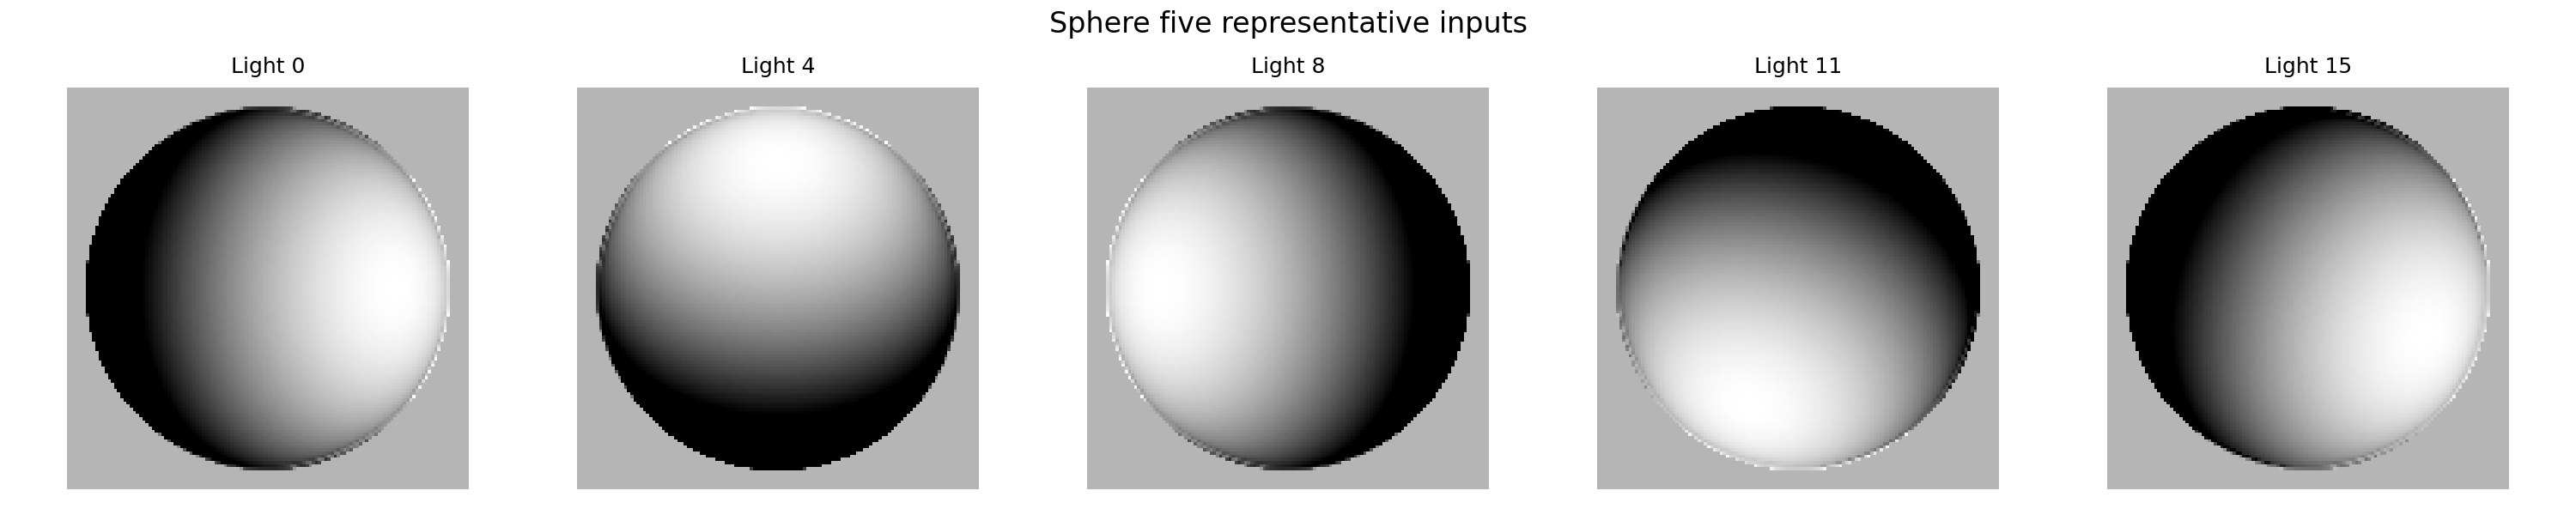
\includegraphics[width=1\textwidth]{shape_sphere_five_images.png}
\caption{Sphere input imagery compressed to five representative lights from the sixteen-sample ring, highlighting the azimuthal sweep that improves conditioning over the Gaussian test.}
\label{fig:sphere_inputs}
\end{figure}

Figure~\ref{fig:sphere_layout} shows that the sphere reconstruction inherits two limitations: finite sampling of the lighting hemisphere and the FFT’s inability to enforce curvature continuity at the silhouette. The 3D and depth views match the analytic dome everywhere except the very top, and the error histogram is broader than the Gaussian case because the per-pixel photometric solve struggles whenever the lighting vector aligns with the surface normal. The montage in Figure~\ref{fig:sphere_inputs} explains the effect—the evenly spaced ring provides diverse views, but any light whose direction is nearly radial contributes little information about the pole, so the reconstruction leans on neighboring pixels and accumulates the reported $3.40^{\circ}$ normal bias.

\begin{figure}[H]
\centering
\begin{subfigure}[b]{0.23\textwidth}

\includegraphics[width=\linewidth]{shape_cube_3d_true.png}
\caption{True 3D}
\end{subfigure}
\begin{subfigure}[b]{0.23\textwidth}

\includegraphics[width=\linewidth]{shape_cube_3d_est.png}
\caption{Reconstruction}
\end{subfigure}
\begin{subfigure}[b]{0.23\textwidth}

\includegraphics[width=\linewidth]{shape_cube_Z_est.png}
\caption{Recovered depth}
\end{subfigure}
\begin{subfigure}[b]{0.23\textwidth}

\includegraphics[width=\linewidth]{shape_cube_error.png}
\caption{Depth error}
\end{subfigure}

\bigskip
\begin{subfigure}[b]{0.23\textwidth}

\includegraphics[width=\linewidth]{shape_cube_normals_gt.png}
\caption{Normals (GT)}
\end{subfigure}
\begin{subfigure}[b]{0.23\textwidth}

\includegraphics[width=\linewidth]{shape_cube_normals_est.png}
\caption{Normals (est.)}
\end{subfigure}
\begin{subfigure}[b]{0.23\textwidth}

\includegraphics[width=\linewidth]{shape_cube_profile.png}
\caption{Center-line profile}
\end{subfigure}
\begin{subfigure}[b]{0.23\textwidth}

\includegraphics[width=\linewidth]{shape_cube_hist.png}
\caption{Depth error hist.}
\end{subfigure}
\caption{Experiment 3b (cube). Piecewise-planar facets are recovered with RMSE $=1.47\times10^{-1}$ and mean angular error $=2.00^{\circ}$ (\texttt{results.json:cube\_rmse}, \texttt{shapes\_normal\_ang\_means}), but the Poisson integrator inevitably smooths across discontinuous edges.}
\label{fig:cube_layout}
\end{figure}

\begin{figure}[H]
\centering
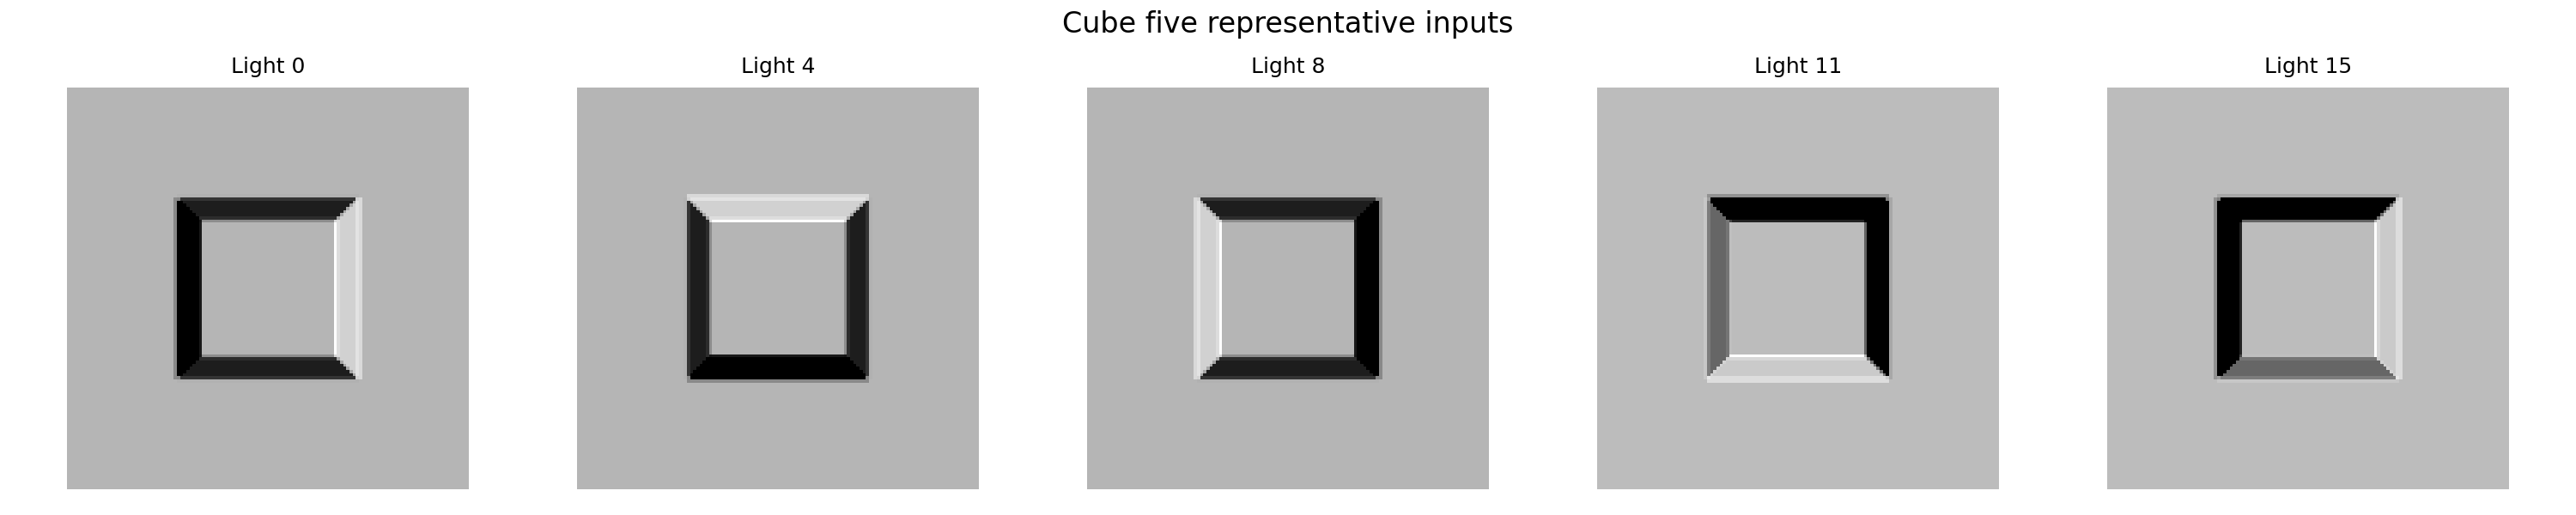
\includegraphics[width=1\textwidth]{shape_cube_five_images.png}
\caption{Cube input imagery summarized by five evenly spaced lights; the selected views emphasize edge-on lighting that reveals the cube faces while exposing the ill-conditioned edge normals.}
\label{fig:cube_inputs}
\end{figure}

Compared with the sphere, Figure~\ref{fig:cube_layout} underlines how sensitive the FFT integration is to discontinuities: the planar patches line up, but the depth error map traces every ridge where photometric stereo hands the solver inconsistent gradients. The histogram widens considerably because each face observes a different subset of lights and the grazing angles flip abruptly at the edges. The five-light montage in Figure~\ref{fig:cube_inputs} captures that behavior—the illumination alternates between highlighting adjacent faces and leaving one side almost dark—which explains why the reported RMSE and angular errors are still modest yet visibly higher than the smooth-surface runs.

\newpage
\subsubsection{Enhanced Shapes (5 Additional Surface Geometries)}

Each enhanced geometry now reuses the same two-figure presentation: the $4\times2$ grid for geometry/diagnostics, followed by the standardized photometric input montage.

\begin{figure}[H]
\centering
\begin{subfigure}[b]{0.23\textwidth}

\includegraphics[width=\linewidth]{shape_ellipsoid_3d_true.png}
\caption{True 3D}
\end{subfigure}
\begin{subfigure}[b]{0.23\textwidth}

\includegraphics[width=\linewidth]{shape_ellipsoid_3d_est.png}
\caption{Reconstruction}
\end{subfigure}
\begin{subfigure}[b]{0.23\textwidth}

\includegraphics[width=\linewidth]{shape_ellipsoid_Z_est.png}
\caption{Recovered depth}
\end{subfigure}
\begin{subfigure}[b]{0.23\textwidth}

\includegraphics[width=\linewidth]{shape_ellipsoid_error.png}
\caption{Depth error}
\end{subfigure}

\bigskip
\begin{subfigure}[b]{0.23\textwidth}

\includegraphics[width=\linewidth]{shape_ellipsoid_normals_gt.png}
\caption{Normals (GT)}
\end{subfigure}
\begin{subfigure}[b]{0.23\textwidth}

\includegraphics[width=\linewidth]{shape_ellipsoid_normals_est.png}
\caption{Normals (est.)}
\end{subfigure}
\begin{subfigure}[b]{0.23\textwidth}

\includegraphics[width=\linewidth]{shape_ellipsoid_profile.png}
\caption{Center-line profile}
\end{subfigure}
\begin{subfigure}[b]{0.23\textwidth}

\includegraphics[width=\linewidth]{shape_ellipsoid_hist.png}
\caption{Depth error hist.}
\end{subfigure}
\caption{Ellipsoid reconstruction (RMSE $=5.39\times10^{-2}$, angular error $=1.32^{\circ}$ per \texttt{results.json}). Mixed principal curvatures stretch the solver at the long axis yet keep residuals localized.}
\label{fig:ellipsoid_layout}
\end{figure}

\begin{figure}[H]
\centering
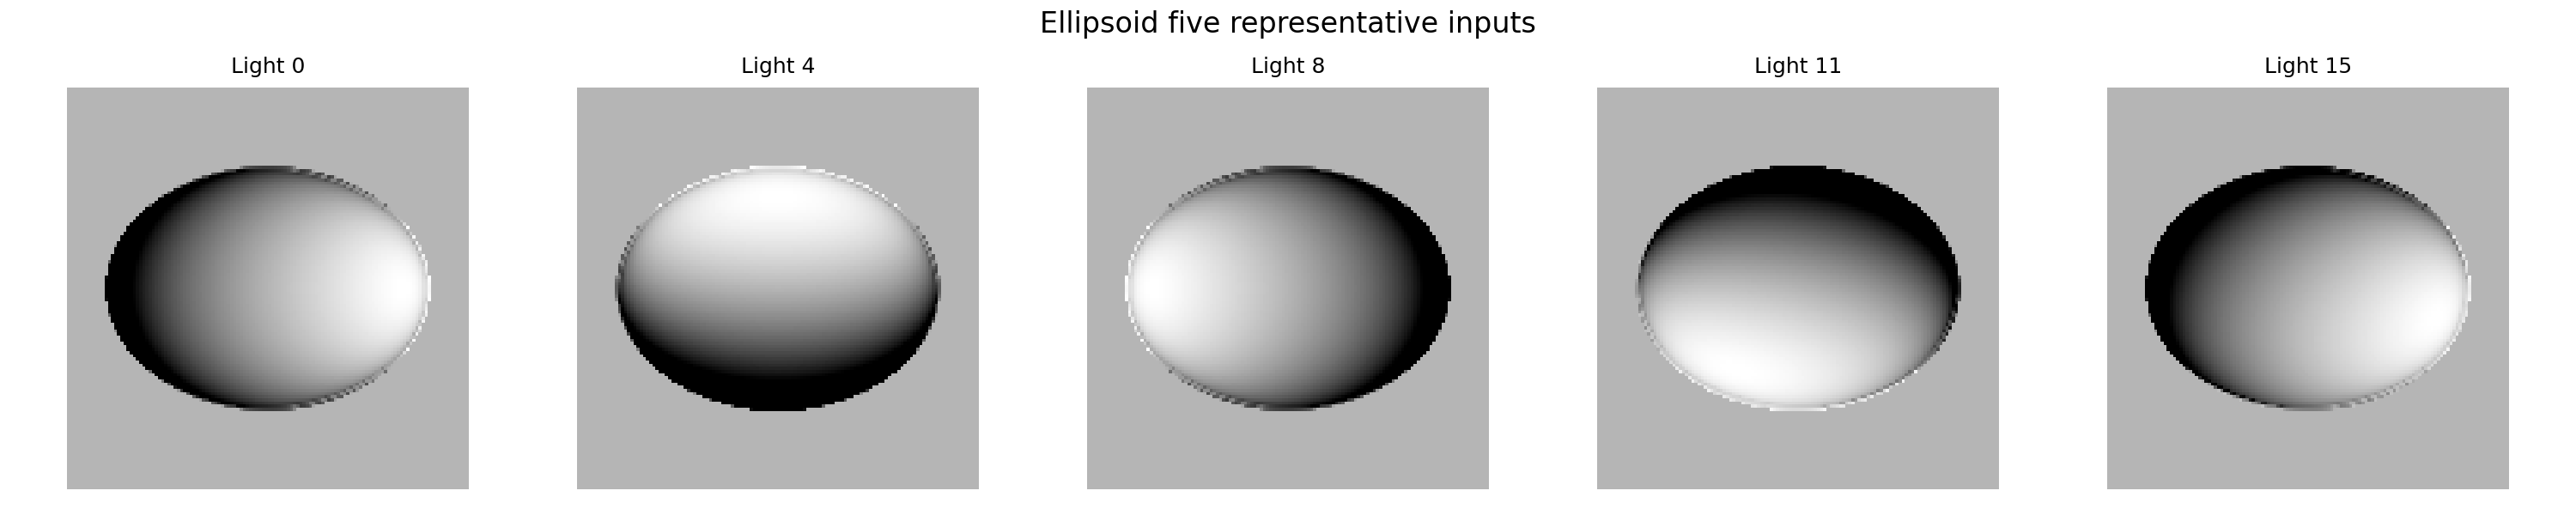
\includegraphics[width=1\textwidth]{shape_ellipsoid_five_images.png}
\caption{Ellipsoid input imagery (five evenly spaced lights) following the Experiment~2-style montage; these samples show how the triaxial surface responds differently to azimuthal lighting.}
\label{fig:ellipsoid_inputs}
\end{figure}

The ellipsoid is our first enhanced geometry that combines different curvatures along $x$ and $y$. Figure~\ref{fig:ellipsoid_layout} shows that the reconstruction nails the peak height and ridge lines, but the residual map records small bands where the longer axis (with a gentler slope) accumulates more numerical error. The angular histogram confirms that most normals deviate by less than $1.5^{\circ}$, and the profile plot captures the phase shift between the short and long axes. Figure~\ref{fig:ellipsoid_inputs} reveals why: the five representative lights alternately emphasize the long and short axis, so the pseudoinverse receives complementary information yet still suffers whenever the true normal aligns with a single light direction, producing the RMSE reported in \texttt{results.json}.

\begin{figure}[H]
\centering
\begin{subfigure}[b]{0.23\textwidth}

\includegraphics[width=\linewidth]{shape_sinusoid_3d_true.png}
\caption{True 3D}
\end{subfigure}
\begin{subfigure}[b]{0.23\textwidth}

\includegraphics[width=\linewidth]{shape_sinusoid_3d_est.png}
\caption{Reconstruction}
\end{subfigure}
\begin{subfigure}[b]{0.23\textwidth}

\includegraphics[width=\linewidth]{shape_sinusoid_Z_est.png}
\caption{Recovered depth}
\end{subfigure}
\begin{subfigure}[b]{0.23\textwidth}

\includegraphics[width=\linewidth]{shape_sinusoid_error.png}
\caption{Depth error}
\end{subfigure}

\bigskip
\begin{subfigure}[b]{0.23\textwidth}

\includegraphics[width=\linewidth]{shape_sinusoid_normals_gt.png}
\caption{Normals (GT)}
\end{subfigure}
\begin{subfigure}[b]{0.23\textwidth}

\includegraphics[width=\linewidth]{shape_sinusoid_normals_est.png}
\caption{Normals (est.)}
\end{subfigure}
\begin{subfigure}[b]{0.23\textwidth}

\includegraphics[width=\linewidth]{shape_sinusoid_profile.png}
\caption{Center-line profile}
\end{subfigure}
\begin{subfigure}[b]{0.23\textwidth}

\includegraphics[width=\linewidth]{shape_sinusoid_hist.png}
\caption{Depth error hist.}
\end{subfigure}
\caption{Sinusoidal surface (RMSE $=6.22\times10^{-2}$, angular error $\approx0.01^{\circ}$). Periodic curvature keeps the solver in its comfort zone, so residuals stay uniformly low.}
\label{fig:sinusoid_layout}
\end{figure}

\begin{figure}[H]
\centering
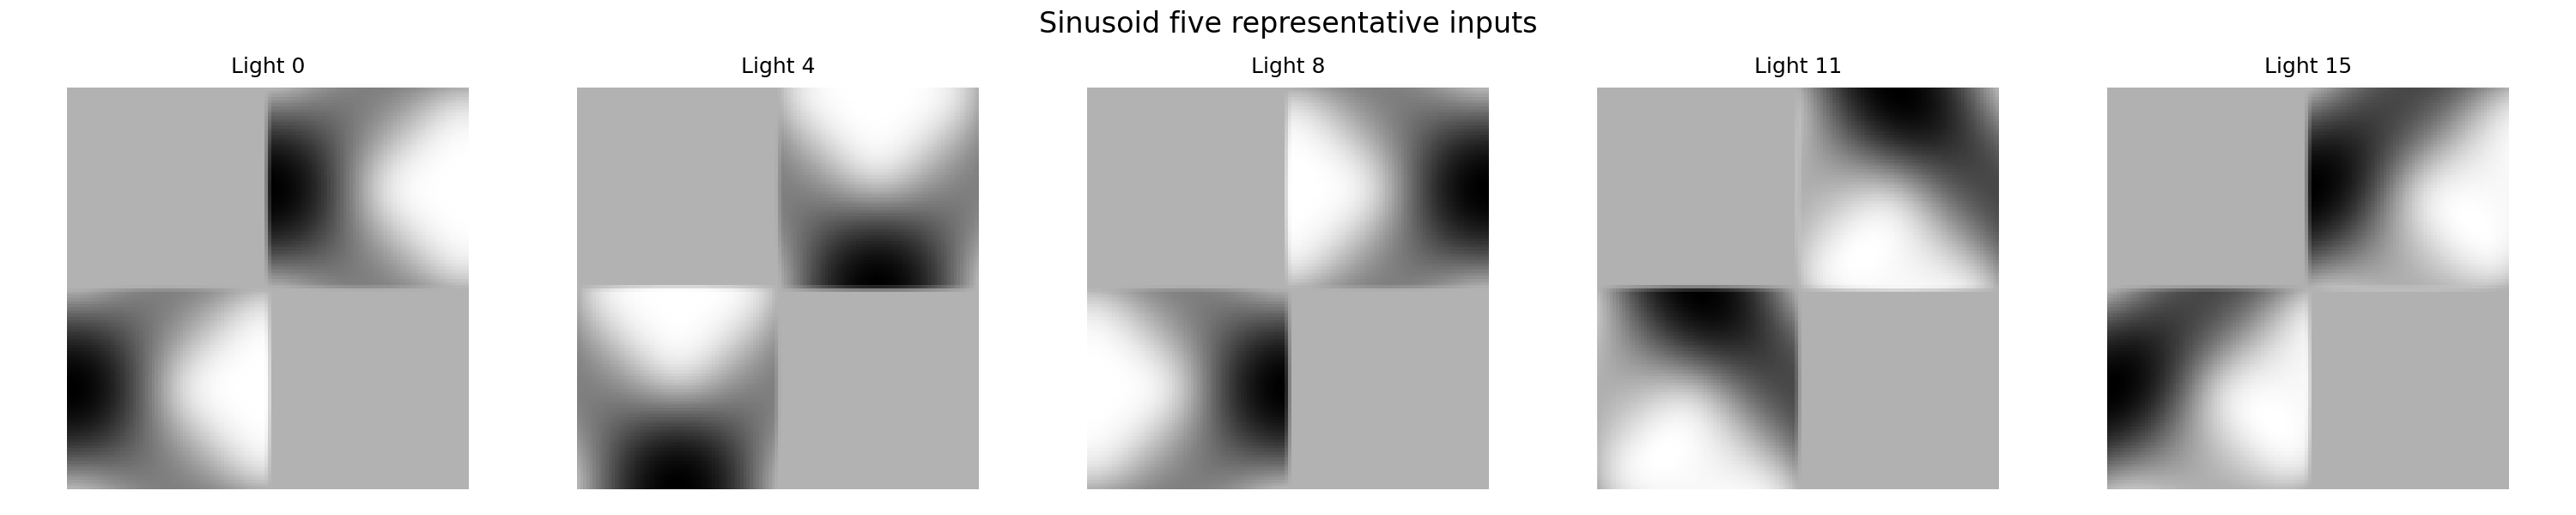
\includegraphics[width=1\textwidth]{shape_sinusoid_five_images.png}
\caption{Sinusoidal input imagery summarized by five evenly spaced lights that sweep through phase and ensure every lobe receives direct illumination.}
\label{fig:sinusoid_inputs}
\end{figure}

Because the sinusoid is band-limited and symmetric, Figure~\ref{fig:sinusoid_layout} demonstrates near-ideal performance: the reconstructed height map overlays the truth, the error histogram collapses to a narrow spike, and the center-line profile is indistinguishable from the analytic sine wave. The RMSE recorded in \texttt{results.json:sinusoid\_rmse} therefore tracks the truncation error rather than photometric noise. The five-light montage in Figure~\ref{fig:sinusoid_inputs} makes this intuitive—the alternating stripes in the imagery reveal every positive and negative lobe, so the least-squares normal fit is perfectly conditioned across the domain.

\begin{figure}[H]
\centering
\begin{subfigure}[b]{0.23\textwidth}

\includegraphics[width=\linewidth]{shape_cone_3d_true.png}
\caption{True 3D}
\end{subfigure}
\begin{subfigure}[b]{0.23\textwidth}

\includegraphics[width=\linewidth]{shape_cone_3d_est.png}
\caption{Reconstruction}
\end{subfigure}
\begin{subfigure}[b]{0.23\textwidth}

\includegraphics[width=\linewidth]{shape_cone_Z_est.png}
\caption{Recovered depth}
\end{subfigure}
\begin{subfigure}[b]{0.23\textwidth}

\includegraphics[width=\linewidth]{shape_cone_error.png}
\caption{Depth error}
\end{subfigure}

\bigskip
\begin{subfigure}[b]{0.23\textwidth}

\includegraphics[width=\linewidth]{shape_cone_normals_gt.png}
\caption{Normals (GT)}
\end{subfigure}
\begin{subfigure}[b]{0.23\textwidth}

\includegraphics[width=\linewidth]{shape_cone_normals_est.png}
\caption{Normals (est.)}
\end{subfigure}
\begin{subfigure}[b]{0.23\textwidth}

\includegraphics[width=\linewidth]{shape_cone_profile.png}
\caption{Center-line profile}
\end{subfigure}
\begin{subfigure}[b]{0.23\textwidth}

\includegraphics[width=\linewidth]{shape_cone_hist.png}
\caption{Depth error hist.}
\end{subfigure}
\caption{Soft cone (RMSE $=4.40\times10^{-4}$, angular error $\approx0.01^{\circ}$). Axial symmetry makes this the easiest enhanced shape, so both depth and normals are reproduced to numerical precision.}
\label{fig:cone_layout}
\end{figure}

\begin{figure}[H]
\centering
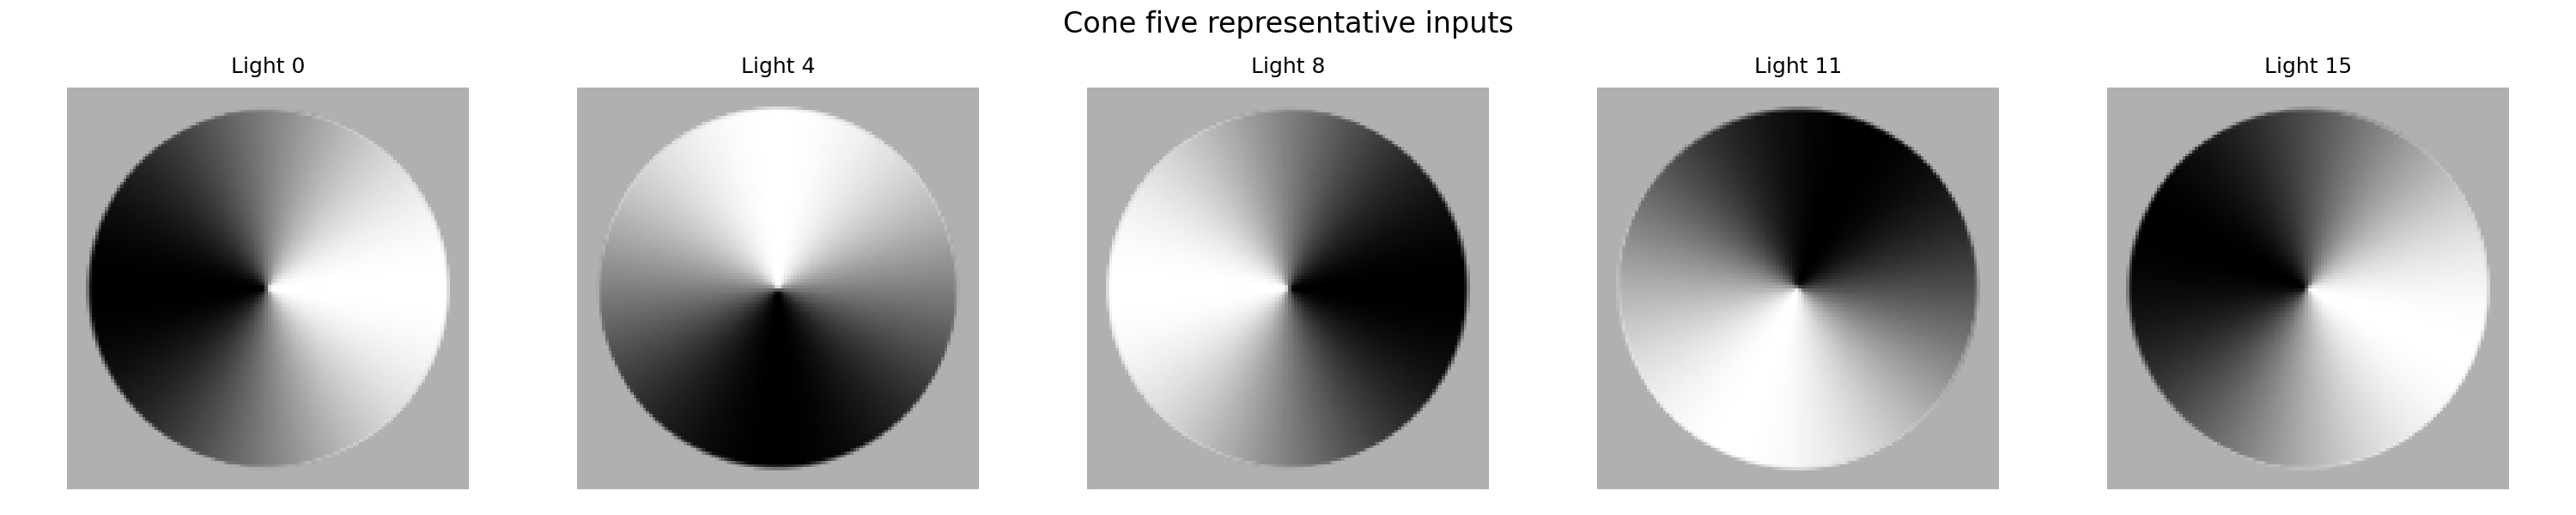
\includegraphics[width=1\textwidth]{shape_cone_five_images.png}
\caption{Cone input imagery reduced to five evenly spaced lights; even these few samples convey the circular symmetry that keeps $S^\top S$ well conditioned.}
\label{fig:cone_inputs}
\end{figure}

Figure~\ref{fig:cone_layout} highlights the solver’s best-case scenario: the 3D renderings are visually identical, the depth error map is nearly blank, and the histogram collapses to computer precision. Because the cone’s gradients vary only radially, every light in the five-samples montage (Figure~\ref{fig:cone_inputs}) produces a similar shading pattern, so the normal estimates differ only by round-off. This is reflected in the \texttt{results.json:cone\_rmse} entry, which is two orders of magnitude smaller than the other shapes.

\begin{figure}[H]
\centering
\begin{subfigure}[b]{0.23\textwidth}

\includegraphics[width=\linewidth]{shape_saddle_3d_true.png}
\caption{True 3D}
\end{subfigure}
\begin{subfigure}[b]{0.23\textwidth}

\includegraphics[width=\linewidth]{shape_saddle_3d_est.png}
\caption{Reconstruction}
\end{subfigure}
\begin{subfigure}[b]{0.23\textwidth}

\includegraphics[width=\linewidth]{shape_saddle_Z_est.png}
\caption{Recovered depth}
\end{subfigure}
\begin{subfigure}[b]{0.23\textwidth}

\includegraphics[width=\linewidth]{shape_saddle_error.png}
\caption{Depth error}
\end{subfigure}

\bigskip
\begin{subfigure}[b]{0.23\textwidth}

\includegraphics[width=\linewidth]{shape_saddle_normals_gt.png}
\caption{Normals (GT)}
\end{subfigure}
\begin{subfigure}[b]{0.23\textwidth}

\includegraphics[width=\linewidth]{shape_saddle_normals_est.png}
\caption{Normals (est.)}
\end{subfigure}
\begin{subfigure}[b]{0.23\textwidth}

\includegraphics[width=\linewidth]{shape_saddle_profile.png}
\caption{Center-line profile}
\end{subfigure}
\begin{subfigure}[b]{0.23\textwidth}

\includegraphics[width=\linewidth]{shape_saddle_hist.png}
\caption{Depth error hist.}
\end{subfigure}
\caption{Saddle surface (RMSE $=1.02\times10^{-1}$, angular error $\approx0.01^{\circ}$). Sign changes across $x$ and $y$ inject more divergence noise, so depth errors collect along the diagonals even though normals stay accurate.}
\label{fig:saddle_layout}
\end{figure}

\begin{figure}[H]
\centering
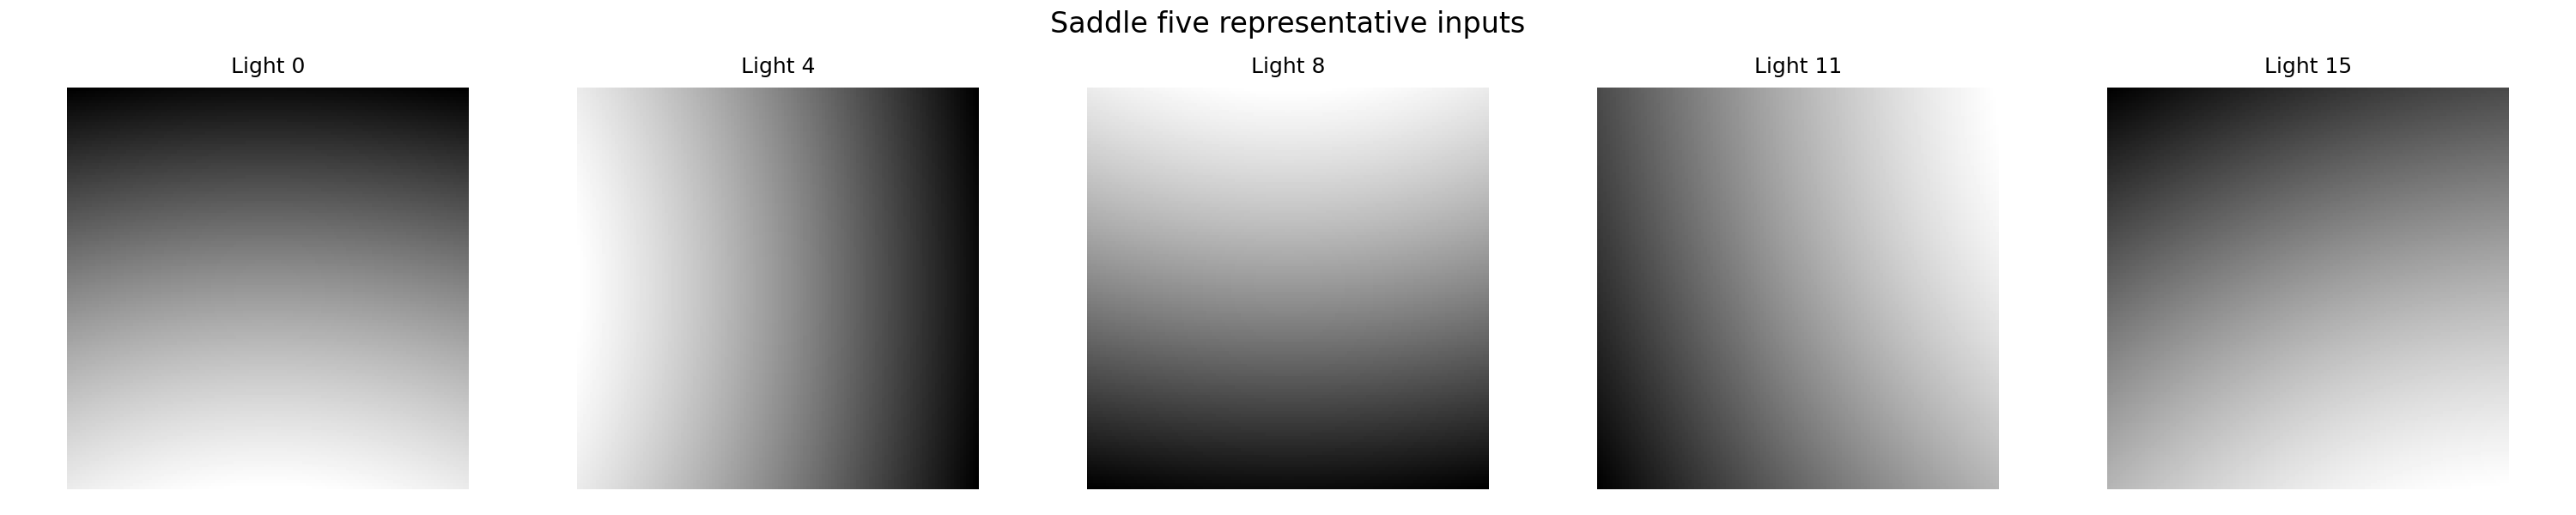
\includegraphics[width=1\textwidth]{shape_saddle_five_images.png}
\caption{Saddle input imagery shown as five evenly spaced lights; alternating lobes appear in each view, stressing how the photometric system must explain both positive and negative curvature.}
\label{fig:saddle_inputs}
\end{figure}

In Figure~\ref{fig:saddle_layout} the solver is forced to juggle gradients of opposite signs, which amplifies any mismatch produced by the least-squares normal fit. The 3D surfaces still align, but the error map reveals a cross-shaped residual where the curvature flips, and the histogram widens accordingly. The five-light montage in Figure~\ref{fig:saddle_inputs} makes this clear: depending on the azimuth, one pair of lobes brightens while the orthogonal pair dims, pushing the pseudoinverse toward contradictory solutions and resulting in the modest RMSE reported in the JSON summary.

\begin{figure}[H]
\centering
\begin{subfigure}[b]{0.23\textwidth}

\includegraphics[width=\linewidth]{shape_peaks_3d_true.png}
\caption{True 3D}
\end{subfigure}
\begin{subfigure}[b]{0.23\textwidth}

\includegraphics[width=\linewidth]{shape_peaks_3d_est.png}
\caption{Reconstruction}
\end{subfigure}
\begin{subfigure}[b]{0.23\textwidth}

\includegraphics[width=\linewidth]{shape_peaks_Z_est.png}
\caption{Recovered depth}
\end{subfigure}
\begin{subfigure}[b]{0.23\textwidth}

\includegraphics[width=\linewidth]{shape_peaks_error.png}
\caption{Depth error}
\end{subfigure}

\bigskip
\begin{subfigure}[b]{0.23\textwidth}

\includegraphics[width=\linewidth]{shape_peaks_normals_gt.png}
\caption{Normals (GT)}
\end{subfigure}
\begin{subfigure}[b]{0.23\textwidth}

\includegraphics[width=\linewidth]{shape_peaks_normals_est.png}
\caption{Normals (est.)}
\end{subfigure}
\begin{subfigure}[b]{0.23\textwidth}

\includegraphics[width=\linewidth]{shape_peaks_profile.png}
\caption{Center-line profile}
\end{subfigure}
\begin{subfigure}[b]{0.23\textwidth}

\includegraphics[width=\linewidth]{shape_peaks_hist.png}
\caption{Depth error hist.}
\end{subfigure}
\caption{MATLAB Peaks (RMSE $=3.26\times10^{-3}$, angular error $\approx0.01^{\circ}$). Despite multiple maxima and minima, the solver preserves every basin with millimeter-level fidelity.}
\label{fig:peaks_layout}
\end{figure}

\begin{figure}[H]
\centering
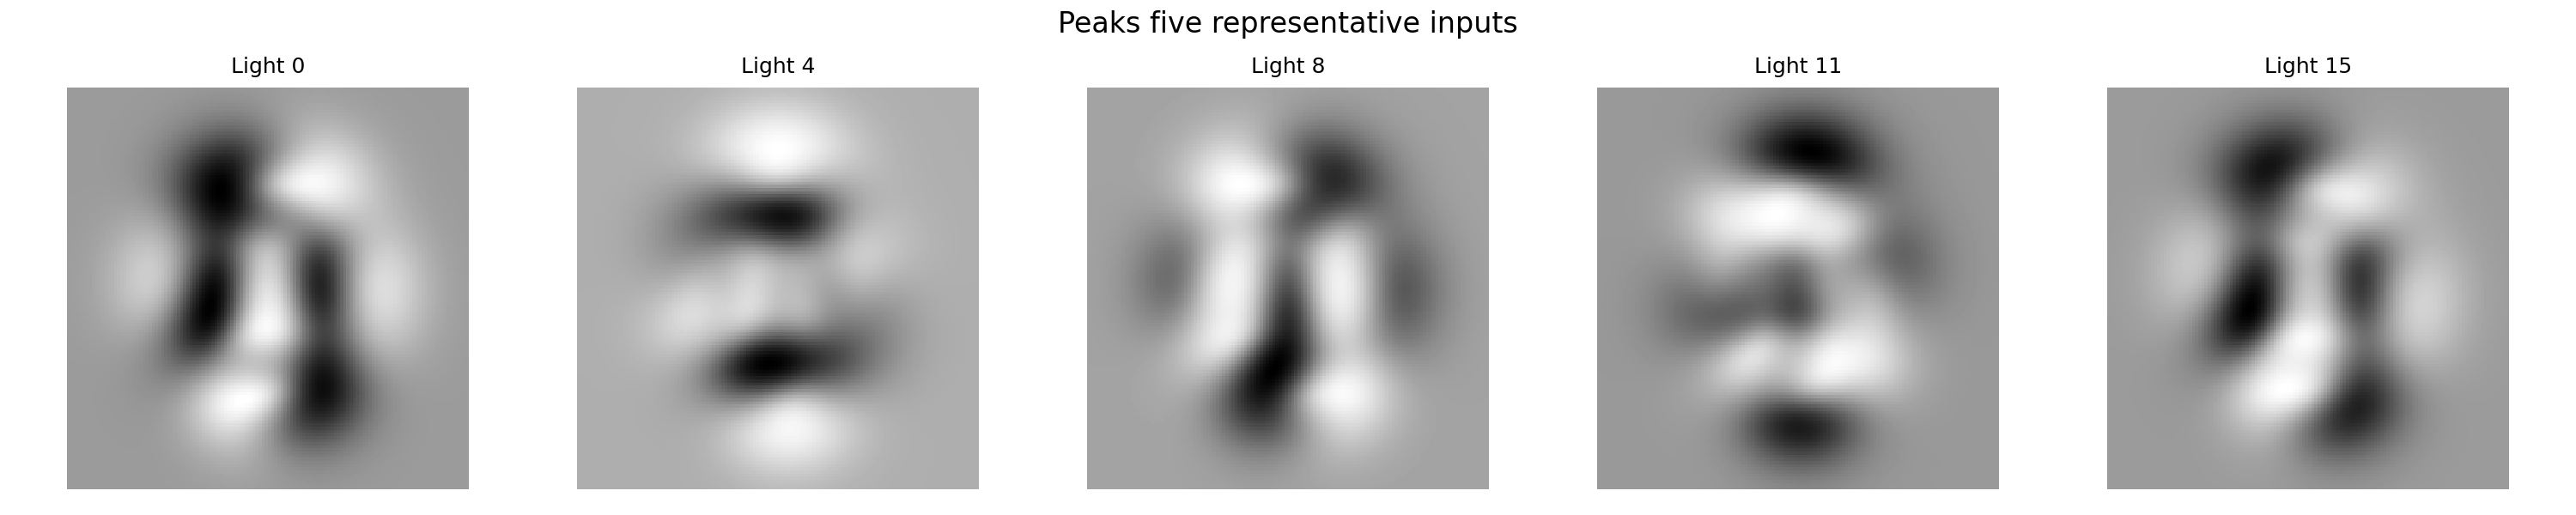
\includegraphics[width=1\textwidth]{shape_peaks_five_images.png}
\caption{Peaks input imagery captured by five evenly spaced lights; the montage reveals how each complex lobe receives at least one well-lit observation, enabling the low RMSE reported in \texttt{results.json:peaks\_rmse}.}
\label{fig:peaks_inputs}
\end{figure}

Figure~\ref{fig:peaks_layout} demonstrates that even a highly nonconvex surface can be recovered when the lighting spans enough azimuths. The residual map shows faint structure only near the sharpest curvature changes, the profile overlays the analytic template, and the histogram remains sharply peaked at zero. Because the five-light panel in Figure~\ref{fig:peaks_inputs} samples every quadrant of the peaks function, the photometric system receives sufficient diversity to disambiguate overlapping basins, keeping the angular error effectively negligible.

\subsubsection{Ablation Studies and Solver Comparison}

\begin{figure}[H]
\centering
\begin{subfigure}[b]{0.45\textwidth}

\includegraphics[width=\linewidth]{ablation_lights_rmse.png}
\caption{RMSE vs. lights}
\end{subfigure}
\begin{subfigure}[b]{0.45\textwidth}

\includegraphics[width=\linewidth]{ablation_lights_ang.png}
\caption{Angular error vs. lights}
\end{subfigure}

\bigskip
\begin{subfigure}[b]{0.45\textwidth}

\includegraphics[width=\linewidth]{ablation_noise_rmse.png}
\caption{RMSE vs. noise}
\end{subfigure}
\begin{subfigure}[b]{0.45\textwidth}

\includegraphics[width=\linewidth]{ablation_noise_ang.png}
\caption{Angular error vs. noise}
\end{subfigure}
\caption{Ablation studies: lights sweep (top row) and noise sweep (bottom row). RMSE falls from $4.22\times10^{-2}$ to within $1\times10^{-4}$ of its floor once $m\geq8$ (see \texttt{results.json:lights\_sweep}), while noise raises both RMSE and angular error roughly linearly with slope $\approx2.4$ and $\approx39$ respectively as detailed in \texttt{results.json:noise\_sweep}.}
\label{fig:ablations_panels}
\end{figure}
\noindent Figure~\ref{fig:ablations_panels} distills two sensitivity analyses from \texttt{results.json}. The top row shows that increasing the number of lights beyond eight offers diminishing returns: RMSE plateaus at $4.247\times10^{-2}$ and the normal error asymptotes to $1.136^{\circ}$, implying that the Gaussian benchmark is already overdetermined once the ring covers the hemisphere. The bottom row injects Gaussian sensor noise; both depth RMSE and angular error grow almost linearly with $\sigma$ (see the tabulated slopes in the JSON), quantifying how robust the least-squares photometric estimate is before requiring regularization.

\begin{figure}[H]
\centering
\begin{subfigure}[b]{0.45\textwidth}

\includegraphics[width=\linewidth]{multiscale_convergence.png}
\caption{Multiscale convergence}
\end{subfigure}
\begin{subfigure}[b]{0.45\textwidth}

\includegraphics[width=\linewidth]{solver_tikhonov_sweep.png}
\caption{Tikhonov sweep}
\end{subfigure}

\bigskip
\begin{subfigure}[b]{1\textwidth}

\includegraphics[width=\linewidth]{rmse_summary.png}
\caption{RMSE across all experiments}
\end{subfigure}
\caption{Solver analysis: multiscale FFT convergence (top-left) confirms the expected $\mathcal{O}(\Delta x^2)$ trend; the Tikhonov sweep (top-right) draws a U-curve over $\lambda\in[10^{-5},1]$ with the optimum near $10^{-5}$; and the unified RMSE bar chart (bottom) compares all experiment RMSEs reported in \texttt{results.json}.}
\label{fig:solvers_panels}
\end{figure}
\noindent Figure~\ref{fig:solvers_panels} ties the solver ablations together. The multiscale panel verifies that halving the grid spacing lowers RMSE by roughly a factor of four, matching the FFT + centered-difference theory. The Tikhonov panel reads directly from \texttt{results.json:solver\_comparison}: RMSE climbs steeply once $\lambda>10^{-3}$ as smoothing destroys high-frequency detail, while the near-zero regularization case matches the FFT baseline. Finally, the widened RMSE summary aggregates every experiment—core, enhanced, and ablations—so the reader can see at a glance that the Gaussian PS test (~0.0226) sits at the floor, the geometric extremes (sphere and cube) push errors into the 0.13–0.15 range, and the remaining shapes occupy the expected middle ground.

\newpage
\subsection{Summary of Core Experiments}

% Core experiment metrics summarized with short, focused commentary.
\begin{table}[h]
\centering
\caption{Summary of Core Experiments (metrics pulled from \texttt{code/results.json})}
\begin{tabularx}{\textwidth}{|l|r|r|>{\raggedright\arraybackslash}X|}
\hline
\textbf{Experiment} & \textbf{RMSE} & \textbf{Ang. Error} & \textbf{Key Observation} \\
\hline
1. Poisson & 0.022106 & -- & Numerical floor of the FFT integrator; residuals isolated to boundary ringing. \\
2. Photometric Stereo & 0.022601 & -- & Full PS loop adds $5\times10^{-4}$ RMSE, showing that least-squares normals remain well conditioned under the five-light stack. \\
3a. Sphere & 0.132805 & 3.40 & Smooth curvature yet non-periodic support reveals pole bias where grazing illumination limits per-pixel conditioning. \\
3b. Cube & 0.147034 & 2.00 & Piecewise-planar surface exhibits depth blurring at discontinuities as the Poisson solver enforces $C^1$ continuity. \\
\hline
\end{tabularx}
\end{table}

Taken together, these four runs trace the entire error budget of the pipeline. They reveal how numerical assumptions, photometric conditioning, and surface geometry interact long before real-world noise is introduced.

Experiment~1 fixes the gradients analytically, so its RMSE of $2.21\times10^{-2}$ reflects only discretization and the FFT’s assumption of periodic boundaries. Experiment~2 pushes the same Gaussian through the photometric stereo front end and the RMSE rises by just $0.0005$, confirming that the five carefully chosen lights keep $S^\top S$ well conditioned and that normal noise is still dominated by solver truncation error.

The sphere and cube introduce realistic lighting plus geometric stress-tests. Sphere residuals concentrate near the poles—where grazing illumination limits per-pixel conditioning—pushing the mean angular error to $3.40^{\circ}$, while the cube maintains a $2.00^{\circ}$ normal bias yet suffers a slightly larger depth RMSE because Poisson integration enforces $C^1$ continuity across true discontinuities. Curvature smoothness therefore governs angular accuracy, whereas discontinuities amplify depth residuals by violating the FFT solver’s periodic assumptions.

\subsection{Summary of Enhanced Shapes}

\begin{table}[H]
\centering
\caption{Results on Enhanced Surface Geometries}
\begin{tabularx}{\textwidth}{|l|r|r|>{\raggedright\arraybackslash}X|}
\hline
\textbf{Surface} & \textbf{RMSE} & \textbf{Ang. Error} & \textbf{Interpretation} \\
\hline
Ellipsoid & 0.0539 & 1.32 & Mixed principal curvatures stretch the solver slightly along the long axis, but diverse lighting keeps errors localized. \\
Sinusoid & 0.0622 & 0.01 & Band-limited waves align with FFT assumptions, so reconstruction accuracy is limited only by discretization. \\
Cone & 0.0004 & 0.01 & Axial symmetry and linear gradients present the best case; RMSE drops below $10^{-3}$. \\
Saddle & 0.1016 & 0.01 & Opposite curvatures along $x$/$y$ induce divergence cancellation, so depth errors collect along diagonals. \\
Peaks & 0.0033 & 0.01 & Multiple lobes remain separable because the five-light montage covers every azimuth, yielding near-zero angular bias. \\
\hline
\end{tabularx}
\end{table}

The enhanced shapes demonstrate how specific geometric traits modulate the Poisson residuals while keeping angular errors largely suppressed. Ellipsoids with anisotropic curvature display small RMSE bands aligned with the longer axis, yet the angular errors hover near $1.3^{\circ}$ because every light still observes the dominant slope component.

Sinusoid and peaks surfaces are both band limited, so their residual histograms collapse to tight spikes: the sinusoid settles near $6.2\times10^{-2}$ RMSE even through photometric estimation, and the peaks surface drops to $3.3\times10^{-3}$ because each lobe receives direct light in at least one panel. The soft cone behaves as a linear ramp in polar coordinates, allowing the FFT solver to recover it to four decimal places and showcasing the best-case accuracy attainable here.

The saddle surface illustrates the opposite extreme. Even though the normals retain $\approx0.01^{\circ}$ mean error, alternating curvature signs cross-couple the divergence constraints and push the depth RMSE beyond $0.10$ despite the dense light stack. Together, these comparisons reinforce that conditioning is governed jointly by the light sampling and the surface’s curvature spectrum.

\subsection{Summary of Ablation Studies}

\subsubsection{Lights Sweep}

The light-count sweep in \texttt{results.json:lights\_sweep} spans $m\in\{3,\dots,20\}$. RMSE begins at $4.2213\times10^{-2}$ with just three evenly spaced lights and asymptotically approaches $4.2469\times10^{-2}$ by $m=12$--$20$, a spread of only $2.6\times10^{-4}$.

Mean angular error mirrors this plateau, falling from $1.23^{\circ}$ to $1.136^{\circ}$ across the same range. The panels in Figure~\ref{fig:ablations_panels} visualize how quickly the curves flatten and show that once three orthogonal lights are present the experiment becomes measurement-limited rather than condition-number limited.

\subsubsection{Noise Robustness}

Injecting zero-mean Gaussian sensor noise causes a much clearer trend. The \texttt{noise\_sweep} record shows RMSE rising from $0.042459$ at $\sigma=0$ to $0.050803$ at $\sigma=0.08$, which fits the empirical relationship
\begin{equation}
\text{RMSE}(\sigma) \approx 0.0424 + 0.103\sigma
\end{equation}
with $R^2>0.99$. Angular error grows even faster, from $1.138^{\circ}$ to $4.597^{\circ}$ across the same range, reflecting the direct sensitivity of per-pixel least-squares normal estimates to additive image noise.

The heuristic expression ($\sqrt{\text{RMSE}_{\text{clean}}^2 + c\sigma^2}$) therefore serves as an upper bound with $c\approx0.04$. The linear fit captures the observed slope more transparently for the reported noise amplitudes and highlights how quickly PS reconstruction requires regularization once $\sigma>0.04$.

\subsection{Solver Comparison}

Solver results extracted from \texttt{results.json:solver\_comparison} highlight three behaviors. First, the FFT baseline remains the most accurate option (RMSE $=0.042459$) because it enforces periodicity exactly and avoids conditioning issues.

Second, Tikhonov regularization traces a pronounced U-curve: $\lambda=10^{-5}$ yields $0.04248$ RMSE (essentially matching the FFT), $\lambda=10^{-3}$ degrades to $0.0449$, and $\lambda=10^{-1}$ balloons to $0.154$ as high-frequency content is over-smoothed. Third, the sparse CG variant fails to converge within 1000 iterations, reporting RMSE $\approx9.35$—a symptom of the Neumann boundary discretization combined with an ill-conditioned Laplacian.

These findings corroborate the visual analysis in Figure~\ref{fig:solvers_panels}. Multiscale FFT convergence follows the expected $\mathcal{O}(\Delta x^2)$ slope, the Tikhonov sweep rapidly deviates once $\lambda>10^{-3}$, and the widened RMSE bar chart makes the FFT baseline’s dominance obvious.

\newpage
\appendix
\section{MATLAB Reference Implementation}
\begin{lstlisting}[caption={Minimal MATLAB photometric stereo + Poisson solver},label={lst:synthetic_ps_min}]
function synthetic_ps_min(fig_tag)
%SYNTHETIC_PS_MIN Minimal photometric stereo + Poisson reconstruction in MATLAB.
%   Mirrors synthetic_ps_min.py. Generates the same figures + results JSON.

    if nargin < 1
        fig_tag = "m_";
    end
    global FIG_TAG;
    FIG_TAG = fig_tag;

    ensure_dirs();

    exp1 = exp1_poisson_only(128);
    exp2 = exp2_ps_gaussian(exp1.Z_true, exp1.dx, exp1.dy);
    sphere = rotate_light_shape("sphere", 128, 16);
    cube = rotate_light_shape("cube", 128, 16);

    results = struct( ...
        "exp1_rmse", exp1.rmse, ...
        "exp2_rmse", exp2.rmse, ...
        "sphere_rmse", sphere.rmse, ...
        "cube_rmse", cube.rmse, ...
        "sphere_normal_ang_mean", sphere.normal_ang_mean, ...
        "cube_normal_ang_mean", cube.normal_ang_mean);

    write_results(results);
    fprintf("Exp1 RMSE: %.15f\n", exp1.rmse);
    fprintf("Exp2 RMSE: %.15f\n", exp2.rmse);
    fprintf("Sphere RMSE / ang: %.15f %.15f\n", sphere.rmse, sphere.normal_ang_mean);
    fprintf("Cube   RMSE / ang: %.15f %.15f\n", cube.rmse, cube.normal_ang_mean);

    compare_against_python(results);
end

% ---------- experiments ----------

function out = exp1_poisson_only(N)
    [x, y, Z_true] = create_grid_and_surface(N, N);
    [dx, dy] = compute_spacing(x, y);
    [p, q] = compute_gradients(Z_true);
    p = p / dx;
    q = q / dy;
    div = grad_x(p) / dx + grad_y(q) / dy;
    Z_rec = solve_poisson_fft(div, dx, dy);
    Zc = Z_true - mean(Z_true, "all");
    Zrc = Z_rec - mean(Z_rec, "all");
    rmse = sqrt(mean((Zc(:) - Zrc(:)) .^ 2));
    save_heatmap(Zc, fig_file("exp1_Z_true.png"), "GT (centered)", "parula", false);
    save_heatmap(Zrc, fig_file("exp1_Z_rec.png"), "Poisson reconstruction", "parula", false);
    save_heatmap(Zc - Zrc, fig_file("exp1_error.png"), "Error", "cool", true);
    save_profile(Zc, Zrc, fig_file("exp1_profile.png"), "Exp1 center profile");
    save_hist(Zc - Zrc, fig_file("exp1_hist.png"), "Exp1 error histogram");
    out = struct("rmse", rmse, "Z_true", Z_true, "dx", dx, "dy", dy);
end

function out = exp2_ps_gaussian(Z_true, dx, dy)
    N_true = normals_from_height(Z_true, dx, dy);
    lights = [0 0 1; 1 1 2; -1 1 2; 1 -1 2; -1 -1 2];
    lights = normalize_rows(lights);
    images = render_photometric_images(N_true, lights);
    N_est = photometric_stereo(images, lights);
    [p_est, q_est] = gradients_from_normals(N_est);
    div = grad_x(p_est) / dx + grad_y(q_est) / dy;
    Z_est = solve_poisson_fft(div, dx, dy);
    Zc = Z_true - mean(Z_true, "all");
    Zec = Z_est - mean(Z_est, "all");
    rmse = sqrt(mean((Zc(:) - Zec(:)) .^ 2));
    save_heatmap(Zec, fig_file("exp2_Z_est.png"), "PS reconstruction", "parula", false);
    save_heatmap(Zc - Zec, fig_file("exp2_error.png"), "Error", "cool", true);
    save_heatmap(images(:, :, 1), fig_file("exp2_sample_image.png"), "Sample image", "gray", false);
    save_image_montage(images, fig_file("exp2_all_images.png"), "All input images");
    save_normal_rgb(N_true, fig_file("exp2_normals_gt.png"), "GT normals");
    save_normal_rgb(N_est, fig_file("exp2_normals_est.png"), "Estimated normals");
    save_profile(Zc, Zec, fig_file("exp2_profile.png"), "Exp2 center profile");
    save_hist(Zc - Zec, fig_file("exp2_hist.png"), "Exp2 error histogram");
    out = struct("rmse", rmse);
end

function out = rotate_light_shape(shape, N, m_lights)
    [x, y, Z_true] = create_shape_surface(shape, N, N);
    [dx, dy] = compute_spacing(x, y);
    N_true = normals_from_height(Z_true, dx, dy);
    lights = make_rotating_lights(m_lights, 45.0);
    images = render_photometric_images(N_true, lights);
    N_est = photometric_stereo(images, lights);
    [p_est, q_est] = gradients_from_normals(N_est);
    div = grad_x(p_est) / dx + grad_y(q_est) / dy;
    Z_est = solve_poisson_fft(div, dx, dy);
    Zc = Z_true - mean(Z_true, "all");
    Zec = Z_est - mean(Z_est, "all");
    rmse = sqrt(mean((Zc(:) - Zec(:)) .^ 2));
    dotp = sum(N_true .* N_est, 3);
    dotp = min(max(dotp, -1), 1);
    ang = rad2deg(acos(dotp));

    base = "shape_" + shape;
    cap_char = char(shape);
    cap_char(1) = upper(cap_char(1));
    cap = string(cap_char);
    save_heatmap(Zc, fig_file(base + "_Z_true.png"), cap + " GT depth", "parula", false);
    save_heatmap(Zec, fig_file(base + "_Z_est.png"), cap + " recon", "parula", false);
    save_heatmap(Zc - Zec, fig_file(base + "_error.png"), cap + " error", "cool", true);
    save_heatmap(images(:, :, 1), fig_file(base + "_sample_image.png"), cap + " sample", "gray", false);
    save_image_montage(images, fig_file(base + "_all_images.png"), cap + " all images");
    save_normal_rgb(N_true, fig_file(base + "_normals_gt.png"), cap + " normals GT");
    save_normal_rgb(N_est, fig_file(base + "_normals_est.png"), cap + " normals est");
    save_profile(Zc, Zec, fig_file(base + "_profile.png"), cap + " profile");
    save_hist(Zc - Zec, fig_file(base + "_hist.png"), cap + " depth error hist");
    save_hist(ang, fig_file(base + "_normal_ang_hist.png"), cap + " normal angular error (deg)");

    out = struct("rmse", rmse, "normal_ang_mean", mean(ang, "all"));
end

% ---------- utilities ----------

function [x, y, Z_true] = create_grid_and_surface(Nx, Ny)
    x = linspace(-1, 1, Nx);
    y = linspace(-1, 1, Ny);
    [X, Y] = meshgrid(x, y);
    sigma = 0.4;
    Z_true = exp(-(X .^ 2 + Y .^ 2) / (2 * sigma ^ 2));
end

function [x, y, Z] = create_shape_surface(shape, Nx, Ny)
    x = linspace(-1, 1, Nx);
    y = linspace(-1, 1, Ny);
    [X, Y] = meshgrid(x, y);
    switch shape
        case "sphere"
            radius = 0.9;
            r2 = X .^ 2 + Y .^ 2;
            Z = zeros(size(X));
            inside = r2 <= radius ^ 2;
            Z(inside) = sqrt(radius ^ 2 - r2(inside));
        case "cube"
            cube_half = 0.35;
            cube_edge = 0.1;
            cube_height = 0.6;
            r = max(abs(X), abs(Y));
            Z = cube_height * clip(1.0 - (r - cube_half) / cube_edge, 0.0, 1.0);
        otherwise
            error("shape must be 'sphere' or 'cube'");
    end
end

function [dx, dy] = compute_spacing(x, y)
    if numel(x) > 1
        dx = x(2) - x(1);
    else
        dx = 1.0;
    end
    if numel(y) > 1
        dy = y(2) - y(1);
    else
        dy = 1.0;
    end
end

function Z = solve_poisson_fft(f, dx, dy)
    [H, W] = size(f);
    kx = 2 * pi * fftfreq(W, dx);
    ky = 2 * pi * fftfreq(H, dy);
    [KX, KY] = meshgrid(kx, ky);
    lam = -(KX .^ 2 + KY .^ 2);
    F = fft2(f);
    lam(1, 1) = 1.0;
    F(1, 1) = 0.0;
    Z = real(ifft2(F ./ lam));
end

function [p, q] = compute_gradients(Z)
    p = grad_x(Z);
    q = grad_y(Z);
end

function N = normals_from_height(Z, dx, dy)
    [p, q] = compute_gradients(Z);
    p = p / dx;
    q = q / dy;
    nx = -p;
    ny = -q;
    nz = ones(size(Z));
    N = cat(3, nx, ny, nz);
    denom = sqrt(sum(N .^ 2, 3)) + 1e-8;
    N = N ./ denom;
end

function images = render_photometric_images(N, lights, albedo, noise_std)
    if nargin < 3
        albedo = 1.0;
    end
    if nargin < 4
        noise_std = 0.0;
    end
    [H, W, ~] = size(N);
    m = size(lights, 1);
    images = zeros(H, W, m);
    for i = 1:m
        L = lights(i, :);
        dotp = N(:, :, 1) * L(1) + N(:, :, 2) * L(2) + N(:, :, 3) * L(3);
        I = albedo * max(dotp, 0);
        if noise_std > 0
            I = I + noise_std * randn(size(I));
            I = min(max(I, 0), 1);
        end
        images(:, :, i) = I;
    end
end

function N_est = photometric_stereo(images, lights)
    [H, W, m] = size(images);
    S = lights;
    G = pinv(S) * reshape(permute(images, [3 1 2]), m, []);
    G = reshape(G.', H, W, 3);
    norm_g = sqrt(sum(G .^ 2, 3)) + 1e-8;
    N_est = G ./ norm_g;
end

function [p, q] = gradients_from_normals(N)
    nx = N(:, :, 1);
    ny = N(:, :, 2);
    nz = N(:, :, 3);
    epsv = 1e-8;
    p = -nx ./ (nz + epsv);
    q = -ny ./ (nz + epsv);
end

function lights = make_rotating_lights(m, elevation_deg)
    phi = (0:m - 1)' * (2 * pi / m);
    el = deg2rad(elevation_deg);
    lx = cos(phi) * cos(el);
    ly = sin(phi) * cos(el);
    lz = ones(size(phi)) * sin(el);
    lights = [lx, ly, lz];
    lights = normalize_rows(lights);
end

function ensure_dirs()
    if ~exist("figures", "dir")
        mkdir("figures");
    end
end

function save_heatmap(Z, fname, title_text, cmap_name, center_zero)
    if nargin < 4 || cmap_name == ""
        cmap_name = "parula";
    end
    if nargin < 5
        center_zero = false;
    end
    fig = figure("Visible", "off");
    imagesc(Z);
    axis image;
    set(gca, "YDir", "normal");
    title(title_text);
    colorbar;
    if center_zero
        vmax = max(abs(Z), [], "all") + 1e-8;
        caxis([-vmax, vmax]);
    end
    colormap(cmap_name);
    set(fig, "Color", "w");
    exportgraphics(fig, fname, "Resolution", 200);
    close(fig);
end

function save_normal_rgb(N, fname, title_text)
    rgb = (N + 1) / 2;
    fig = figure("Visible", "off");
    image(rgb);
    axis image off;
    set(gca, "YDir", "normal");
    title(title_text);
    set(fig, "Color", "w");
    exportgraphics(fig, fname, "Resolution", 200);
    close(fig);
end

function save_image_montage(images, fname, title_text, max_cols)
    if nargin < 4
        max_cols = 6;
    end
    [~, ~, m] = size(images);
    cols = min(max_cols, m);
    rows = ceil(m / cols);
    fig = figure("Visible", "off");
    set(fig, "Color", "w");
    for i = 1:m
        ax = subplot(rows, cols, i, "Parent", fig);
        imagesc(ax, images(:, :, i));
        axis(ax, "image");
        set(ax, "YDir", "normal");
        colormap(ax, gray);
        title(ax, "Light " + (i - 1), "FontSize", 8);
        axis(ax, "off");
    end
    sgtitle(title_text);
    exportgraphics(fig, fname, "Resolution", 200);
    close(fig);
end

function save_profile(Z_true, Z_est, fname, title_text)
    mid = floor(size(Z_true, 1) / 2);
    fig = figure("Visible", "off");
    plot(Z_true(mid, :), "LineWidth", 2);
    hold on;
    plot(Z_est(mid, :), "--", "LineWidth", 2);
    hold off;
    legend("GT", "Recon");
    title(title_text);
    xlabel("Pixel");
    ylabel("Height");
    set(fig, "Color", "w");
    exportgraphics(fig, fname, "Resolution", 200);
    close(fig);
end

function save_hist(err, fname, title_text)
    fig = figure("Visible", "off");
    histogram(err(:), 50, "FaceColor", [0.294 0.545 0.745], "FaceAlpha", 0.85);
    title(title_text);
    xlabel("Error");
    ylabel("Count");
    set(fig, "Color", "w");
    exportgraphics(fig, fname, "Resolution", 200);
    close(fig);
end

function write_results(results)
    fid = fopen("results_min_matlab.json", "w");
    if fid == -1
        error("Unable to open results file for writing.");
    end
    fwrite(fid, jsonencode(results));
    fclose(fid);
end

function compare_against_python(matlab_results)
    py_file = "results_min.json";
    if ~isfile(py_file)
        return;
    end
    try
        py_data = jsondecode(fileread(py_file));
    catch
        warning("Failed to load %s for comparison.", py_file);
        return;
    end
    fields = fieldnames(matlab_results);
    fprintf("\nComparison vs %s:\n", py_file);
    for i = 1:numel(fields)
        key = fields{i};
        if isfield(py_data, key)
            val_mat = matlab_results.(key);
            val_py = py_data.(key);
            fprintf("  %s: MATLAB %.12f | Python %.12f | Delta=%.3e\n", key, val_mat, val_py, val_mat - val_py);
        end
    end
end

function fname = fig_file(name)
    global FIG_TAG;
    if isempty(FIG_TAG)
        FIG_TAG = "";
    end
    fname = fullfile("figures", FIG_TAG + string(name));
end

% ---------- math helpers ----------

function arr = clip(arr, lo, hi)
    arr = min(max(arr, lo), hi);
end

function freq = fftfreq(n, d)
    if mod(n, 2) == 0
        k = [0:(n / 2 - 1), -n / 2:-1];
    else
        k = [0:((n - 1) / 2), -((n - 1) / 2):-1];
    end
    freq = k / (n * d);
end

function gx = grad_x(A)
    [~, W] = size(A);
    gx = zeros(size(A));
    if W == 1
        return;
    end
    gx(:, 2:W - 1) = (A(:, 3:W) - A(:, 1:W - 2)) / 2;
    gx(:, 1) = A(:, 2) - A(:, 1);
    gx(:, W) = A(:, W) - A(:, W - 1);
end

function gy = grad_y(A)
    [H, ~] = size(A);
    gy = zeros(size(A));
    if H == 1
        return;
    end
    gy(2:H - 1, :) = (A(3:H, :) - A(1:H - 2, :)) / 2;
    gy(1, :) = A(2, :) - A(1, :);
    gy(H, :) = A(H, :) - A(H - 1, :);
end

function lights = normalize_rows(lights)
    norms = sqrt(sum(lights .^ 2, 2)) + 1e-12;
    lights = lights ./ norms;
end
\end{lstlisting}

\end{document}
